\documentclass[dvipdfmx,10pt,aspectratio=169]{beamer}


% figure caption
\usepackage{caption}
\captionsetup[figure]{labelformat=empty}
% font family
\usepackage{helvet}
% use gothic font for japanese
\renewcommand{\kanjifamilydefault}{\gtdefault}


% theme
\usetheme{Madrid}
\usefonttheme{professionalfonts}
\useoutertheme[height=0cm,width=1.5cm,left]{sidebar}


% frame number
\setbeamertemplate{frametitle}{
    \nointerlineskip
    \begin{beamercolorbox}[wd=\paperwidth,ht=2.25ex,dp=0.75ex]{frametitle} % set ht
        \hspace*{1ex}\insertframetitle
        % \hfill\insertframenumber/\inserttotalframenumber\hspace*{8ex}
        \hfill\insertframenumber/{27}\hspace*{8ex}
    \end{beamercolorbox}
}


% hides nvigation buttons at bottom
\setbeamertemplate{navigation symbols}{}


% Remove title and name from sidebar
\makeatletter
\setbeamertemplate{sidebar \beamer@sidebarside}%{sidebar theme}
{
    \beamer@tempdim=\beamer@sidebarwidth%
    \advance\beamer@tempdim by 10pt%
    \insertverticalnavigation{\beamer@sidebarwidth}%
    \vfill
    \ifx\beamer@sidebarside\beamer@lefttext%
    \else%
    \usebeamercolor{normal text}%
    \llap{\usebeamertemplate***{navigation symbols}\hskip0.1cm}%
    \vskip5pt%
    \fi%
}%
\makeatother


% show toc at the beginning of each section
\AtBeginSection[]
{
    \begin{frame}
        \frametitle{目次}
        \tableofcontents[currentsection]
    \end{frame}
}


% display transparently
\setbeamercovered{transparent}


% table style
% This sets the thickness of the borders of the table.
\setlength{\arrayrulewidth}{0.5mm}
% The space between the text and the left/right border of its containing cell
\setlength{\tabcolsep}{18pt}
% The height of each row is set to 1.5 relative to its default height.
\renewcommand{\arraystretch}{2.5}


% define colors
% ---------------------------------------------------------------------------- %
\definecolor{red}{rgb}{0.9,0.30,0.30}
\definecolor{blue}{rgb}{0.32,0.66,0.82}
\definecolor{darkblue}{rgb}{0.2,0.4,0.6}
\definecolor{green}{rgb}{0.47,0.72,0.29}
\definecolor{darkgreen}{rgb}{0.25,0.42,0.21}
\definecolor{yellow}{rgb}{0.95,0.85,0.25}
\definecolor{darkyellow}{rgb}{0.75,0.65,0.05}
\definecolor{orange}{rgb}{0.95,0.55,0.25}
\definecolor{darkorange}{rgb}{0.75,0.35,0.05}
\definecolor{purple}{rgb}{0.75,0.55,0.85}
\definecolor{darkpurple}{rgb}{0.55,0.35,0.65}
\definecolor{brown}{rgb}{0.75,0.55,0.25}
\definecolor{darkbrown}{rgb}{0.55,0.35,0.05}
\definecolor{pink}{rgb}{0.95,0.55,0.75}
\definecolor{darkpink}{rgb}{0.75,0.35,0.55}
\definecolor{grey}{rgb}{0.55,0.55,0.55}
\definecolor{darkgrey}{rgb}{0.35,0.35,0.35}
% ---------------------------------------------------------------------------- %


% set colors
% ---------------------------------------------------------------------------- %
\setbeamercolor{structure}{fg=blue}
\setbeamertemplate{blocks}[rounded][shadow=false]
\setbeamercolor{block title alerted}{bg=red, fg=white}
\setbeamercolor{block title example}{bg=green, fg=white}


% define blocks
% ---------------------------------------------------------------------------- %
\addtobeamertemplate{proof begin}{
    \setbeamercolor{block title}{bg=grey, fg=white}
}{}

\newenvironment<>{note}[1]{
    \setbeamercolor{block title}{bg=blue, fg=white}
    \begin{block}{Note}#1}{\end{block}}
\newenvironment<>{warning}[1]{
    \setbeamercolor{block title}{bg=red}
    \begin{block}{Warning}#1}{\end{block}}
\newenvironment<>{important}[1]{
    \setbeamercolor{block title}{bg=orange}
    \begin{block}{Important}#1}{\end{block}}

\newenvironment<>{theorem}[1]{
    \setbeamercolor{block title}{bg=darkblue, fg=white}
    \begin{block}{定理}#1}{\end{block}}
% \newenvironment<>{proof}[1]{
%     \setbeamercolor{block title}{bg=grey, fg=white}
%     \begin{block}{証明は論文}#1}{\end{block}}
\newenvironment<>{definition}[1]{
    \setbeamercolor{block title}{bg=grey}
    \begin{block}{定義}#1}{\end{block}}
% \newenvironment<>{definition}[1]{
%     \setbeamercolor{block title}{bg=grey}
%     \begin{block}{Definition}#1}{\end{block}}
\newenvironment<>{proposition}[1]{
    \setbeamercolor{block title}{bg=darkblue}
    \begin{block}{Proposition}#1}{\end{block}}
\newenvironment<>{lemma}[1]{
    \setbeamercolor{block title}{bg=darkblue}
    \begin{block}{Lemma}#1}{\end{block}}
\newenvironment<>{corollary}[1]{
    \setbeamercolor{block title}{bg=darkblue}
    \begin{block}{Corollary}#1}{\end{block}}
\newenvironment<>{remark}[1]{
    \setbeamercolor{block title}{bg=blue}
    \begin{block}{Remark}#1}{\end{block}}
% ---------------------------------------------------------------------------- %
% mathtools: math tools, mathrsfs: RSFS fonts
\usepackage{mathtools,mathrsfs}
% physics
\usepackage{physics}
% algorithm
\usepackage{algorithm,algorithmic}
% vector graphics
\usepackage{tikz}
\usetikzlibrary{quantikz}
% comment
\usepackage{comment}
% dummy text
\usepackage{lipsum}
% image position
\usepackage{here}


% latin abbreviations
% ---------------------------------------------------------------------------- %
\newcommand{\etal}{\textit{et al.}}
\newcommand{\eg}{\textit{e.g.}}
\newcommand{\cf}{\textit{c.f.}}
\newcommand{\ie}{\textit{i.e.}}
\newcommand{\etc}{\textit{etc.}}
% ---------------------------------------------------------------------------- %


% math
% ---------------------------------------------------------------------------- %
% mathbb
\newcommand{\bbA}{\mathbb{A}}
\newcommand{\bbB}{\mathbb{B}}
\newcommand{\bbC}{\mathbb{C}}
\newcommand{\bbD}{\mathbb{D}}
\newcommand{\bbE}{\mathbb{E}}
\newcommand{\bbF}{\mathbb{F}}
\newcommand{\bbG}{\mathbb{G}}
\newcommand{\bbH}{\mathbb{H}}
\newcommand{\bbI}{\mathbb{I}}
\newcommand{\bbJ}{\mathbb{J}}
\newcommand{\bbK}{\mathbb{K}}
\newcommand{\bbL}{\mathbb{L}}
\newcommand{\bbM}{\mathbb{M}}
\newcommand{\bbN}{\mathbb{N}}
\newcommand{\bbO}{\mathbb{O}}
\newcommand{\bbP}{\mathbb{P}}
\newcommand{\bbQ}{\mathbb{Q}}
\newcommand{\bbR}{\mathbb{R}}
\newcommand{\bbS}{\mathbb{S}}
\newcommand{\bbT}{\mathbb{T}}
\newcommand{\bbU}{\mathbb{U}}
\newcommand{\bbV}{\mathbb{V}}
\newcommand{\bbW}{\mathbb{W}}
\newcommand{\bbX}{\mathbb{X}}
\newcommand{\bbY}{\mathbb{Y}}
\newcommand{\bbZ}{\mathbb{Z}}

% \mathrm capital letters
\newcommand{\rmA}{\mathrm{A}}
\newcommand{\rmB}{\mathrm{B}}
\newcommand{\rmC}{\mathrm{C}}
\newcommand{\rmD}{\mathrm{D}}
\newcommand{\rmE}{\mathrm{E}}
\newcommand{\rmF}{\mathrm{F}}
\newcommand{\rmG}{\mathrm{G}}
\newcommand{\rmH}{\mathrm{H}}
\newcommand{\rmI}{\mathrm{I}}
\newcommand{\rmJ}{\mathrm{J}}
\newcommand{\rmK}{\mathrm{K}}
\newcommand{\rmL}{\mathrm{L}}
\newcommand{\rmM}{\mathrm{M}}
\newcommand{\rmN}{\mathrm{N}}
\newcommand{\rmO}{\mathrm{O}}
\newcommand{\rmP}{\mathrm{P}}
\newcommand{\rmQ}{\mathrm{Q}}
\newcommand{\rmR}{\mathrm{R}}
\newcommand{\rmS}{\mathrm{S}}
\newcommand{\rmT}{\mathrm{T}}
\newcommand{\rmU}{\mathrm{U}}
\newcommand{\rmV}{\mathrm{V}}
\newcommand{\rmW}{\mathrm{W}}
\newcommand{\rmX}{\mathrm{X}}
\newcommand{\rmY}{\mathrm{Y}}
\newcommand{\rmZ}{\mathrm{Z}}

% \mathcal capital letters
\newcommand{\calA}{\mathcal{A}}
\newcommand{\calB}{\mathcal{B}}
\newcommand{\calC}{\mathcal{C}}
\newcommand{\calD}{\mathcal{D}}
\newcommand{\calE}{\mathcal{E}}
\newcommand{\calF}{\mathcal{F}}
\newcommand{\calG}{\mathcal{G}}
\newcommand{\calH}{\mathcal{H}}
\newcommand{\calI}{\mathcal{I}}
\newcommand{\calJ}{\mathcal{J}}
\newcommand{\calK}{\mathcal{K}}
\newcommand{\calL}{\mathcal{L}}
\newcommand{\calM}{\mathcal{M}}
\newcommand{\calN}{\mathcal{N}}
\newcommand{\calO}{\mathcal{O}}
\newcommand{\calP}{\mathcal{P}}
\newcommand{\calQ}{\mathcal{Q}}
\newcommand{\calR}{\mathcal{R}}
\newcommand{\calS}{\mathcal{S}}
\newcommand{\calT}{\mathcal{T}}
\newcommand{\calU}{\mathcal{U}}
\newcommand{\calV}{\mathcal{V}}
\newcommand{\calW}{\mathcal{W}}
\newcommand{\calX}{\mathcal{X}}
\newcommand{\calY}{\mathcal{Y}}
\newcommand{\calZ}{\mathcal{Z}}

% multiplicative group
\newcommand{\Zx}{\Z^\times}
\newcommand{\Qx}{\Q^\times}
\newcommand{\Rx}{\R^\times}
\newcommand{\Cx}{\C^\times}

% non-negative
\newcommand{\Znn}{\Z_{\ge0}}
\newcommand{\Qnn}{\Q_{\ge0}}
\newcommand{\Rnn}{\R_{\ge0}}

% positive
\newcommand{\Zpo}{\Z_{>0}}
\newcommand{\Qpo}{\Q_{>0}}
\newcommand{\Rpo}{\R_{>0}}

% mathrm
\newcommand{\const}{\mathrm{const}}
\newcommand{\hc}{\mathrm{h.c.}}
\newcommand{\lhs}{\mathrm{(LHS)}}
\newcommand{\rhs}{\mathrm{(RHS)}}
\newcommand{\Haar}{\mathrm{Haar}}
\newcommand{\poly}{\mathrm{poly}}
\newcommand{\SWAP}{\mathrm{SWAP}}

% MathOperator
\DeclareMathOperator*{\argmin}{arg~min}
\DeclareMathOperator*{\argmax}{arg~max}
\DeclareMathOperator{\sgn}{sgn}
\DeclareMathOperator{\sign}{sign}
\DeclareMathOperator{\Supp}{Supp}
\DeclareMathOperator{\diag}{diag}
\DeclareMathOperator{\E}{E}
\DeclareMathOperator{\Var}{Var}
\DeclareMathOperator{\Cov}{Cov}
\DeclareMathOperator{\Hom}{Hom}
\DeclareMathOperator{\Aut}{Aut}
\DeclareMathOperator{\End}{End}

% others
\renewcommand{\bar}[1]{\overline{#1}}
\newcommand{\combi}[2]{{}_{#1}\text{C}_{#2}}
\newcommand{\dg}{^\dagger}
\newcommand{\fa}{{}^\forall}
\newcommand{\ex}{{}^\exists}
\newcommand{\pd}{\partial}
\newcommand*\circled[1]{\tikz[baseline=(char.base)]{
            \node[shape=circle,draw,inner sep=2pt] (char) {#1};}\,}
\newcommand{\bs}[1]{\vb*{#1}}
\newcommand{\bx}{\vb*{x}}
\newcommand{\by}{\vb*{y}}
\newcommand{\bth}{\vb*{\theta}}
\newcommand{\ot}{\otimes}
\newcommand{\otn}[1]{^{\otimes {#1}}}
\newcommand{\kten}[2]{\ket{#1}\otimes\ket{#2}}
\newcommand{\bten}[2]{\bra{#1}\otimes\bra{#2}}
\newcommand{\memo}[1]{\textcolor{red}{(#1)}}
\usepackage{dsfont}
\newcommand{\bbid}{\mathds{1}}
% ---------------------------------------------------------------------------- %


% physics
% ---------------------------------------------------------------------------- %
% matrix
\newcommand{\paulix}{ \mqty(\pmat{1}) }
\newcommand{\pauliy}{ \mqty(\pmat{2}) }
\newcommand{\pauliz}{ \mqty(\pmat{3}) }

\newcommand{\rx}[1]{ \mqty[\cos \frac{#1}{2} & -i\sin\frac{#1}{2} \\ -i\sin \frac{#1}{2}& \cos\frac{#1}{2} ]}
\newcommand{\ry}[1]{ \mqty[\cos \frac{#1}{2} & -\sin\frac{#1}{2}  \\ \sin \frac{#1}{2}  & \cos\frac{#1}{2} ]}
\newcommand{\rz}[1]{ \mqty[e^{-i{#1}/2}      & 0                  \\ 0                  & e^{i{#1}/2}     ]}
\newcommand{\rot}[1]{\mqty[\cos {#1}         & -\sin {#1}         \\ \sin {#1}          & \cos {#1} ]}

% sin cos
\newcommand{\sif}[2]{\sin\qty(\frac{#1}{#2})}
\newcommand{\cof}[2]{\cos\qty(\frac{#1}{#2})}

% spin
\newcommand{\up}{\uparrow} %spin up
\newcommand{\down}{\downarrow} %spin down
\newcommand{\szero}{\mqty( 1 \\ 0 )} %spin zero
\newcommand{\sone}{\mqty( 0 \\ 1 )} %spin one
% ---------------------------------------------------------------------------- %

% ref: https://github.com/SSoelvsten/latex-preamble-and-examples/tree/main/documents
\graphicspath{{../img/}}


\title{量子機械学習におけるデータ符号化由来の\\勾配消失に関する研究}
\author{東京大学 理学系研究科 物理学専攻 寺師研究室 \\上曽山 健介}
\date{2024/01/24}

\begin{document}

\frame{\titlepage}

\begin{frame}{目次}
    \tableofcontents
\end{frame}



\section{前提知識}
\subsection{量子コンピューター}
\begin{frame}{量子コンピューター}
    \begin{center}
        {\large\colorbox{blue!40}{\makebox[15em]{量子コンピューター}}}
    \end{center}
    \begin{columns}
        \begin{column}{0.7\textwidth}
            量子計算を行う量子回路は以下の要素から成る。
            \begin{itemize}
                \item 量子ビット:2準位量子系
                \item 量子ゲート:量子ビットの状態を変化させるユニタリ
                \item 測定   :量子状態から情報を読み出す操作
            \end{itemize}
        \end{column}

        \begin{column}{0.3\textwidth}
            \begin{tikzpicture}
                \node[scale=0.6]{
                \begin{quantikz}
                    \lstick{$\ket{0}$} & \gate{H} & \ctrl{1} &  \qw    & \gate{X} & \meter{} \\
                    \lstick{$\ket{0}$} & \gate{T} & \targ{} & \ctrl{1} & \gate{S} & \meter{} \\
                    \lstick{$\ket{0}$} & \gate{H} &   \qw   & \targ{}  & \gate{H} & \meter{} \\
                \end{quantikz}};
            \end{tikzpicture}
        \end{column}
    \end{columns}

    \begin{center}
        {\large\colorbox{blue!40}{\makebox[27em]{NISQ (Noisy Intermediate-Scale Quantum device) {\small[\href{http://arxiv.org/abs/1801.00862}{Preskill2018}]} }}}
    \end{center}

    \begin{center}
        \begin{minipage}{0.7\textwidth}
            \begin{itemize}
                \item 数百量子ビット程度の規模の量子コンピューター\\
                \item 誤り訂正ができないため、ノイズを無視できない\\
                \item 使用できる量子回路の深さに限界がある
            \end{itemize}
        \end{minipage}
    \end{center}

\end{frame}



\newcommand{\tabitem}{\usebeamertemplate{itemize item}\hspace*{\labelsep}}
\subsection{変分量子アルゴリズム}
\begin{frame}{変分量子アルゴリズム}
    \vspace*{-10pt}
    \begin{center}
        {\large\colorbox{blue!40}{\makebox[17em]{変分量子アルゴリズム} {\small[\href{http://arxiv.org/abs/2012.09265}{review:Cerezo2021}]} }}
    \end{center}

    \begin{center}
        \begin{minipage}{0.8\textwidth}
            \begin{itemize}
                \item NISQで実行可能な量子\&古典ハイブリッドアルゴリズム
                \item $U(\bth)$: パラメーター化された量子回路(変分量子回路)
                \item $\ell_{i,k}(\bth) = \Tr[U(\bth)\rho_i U\dg(\bth)O_k]$、$\rho_i$: 初期状態、$O_k$: オブザーバブル
                \item コスト関数 $\calL(\bth) = f(\{\ell_{i,k}(\bth)\}_{i,k})$ の最適化
                \item 量子化学計算、組み合わせ最適化、機械学習などに応用
            \end{itemize}
        \end{minipage}
    \end{center}

    \centering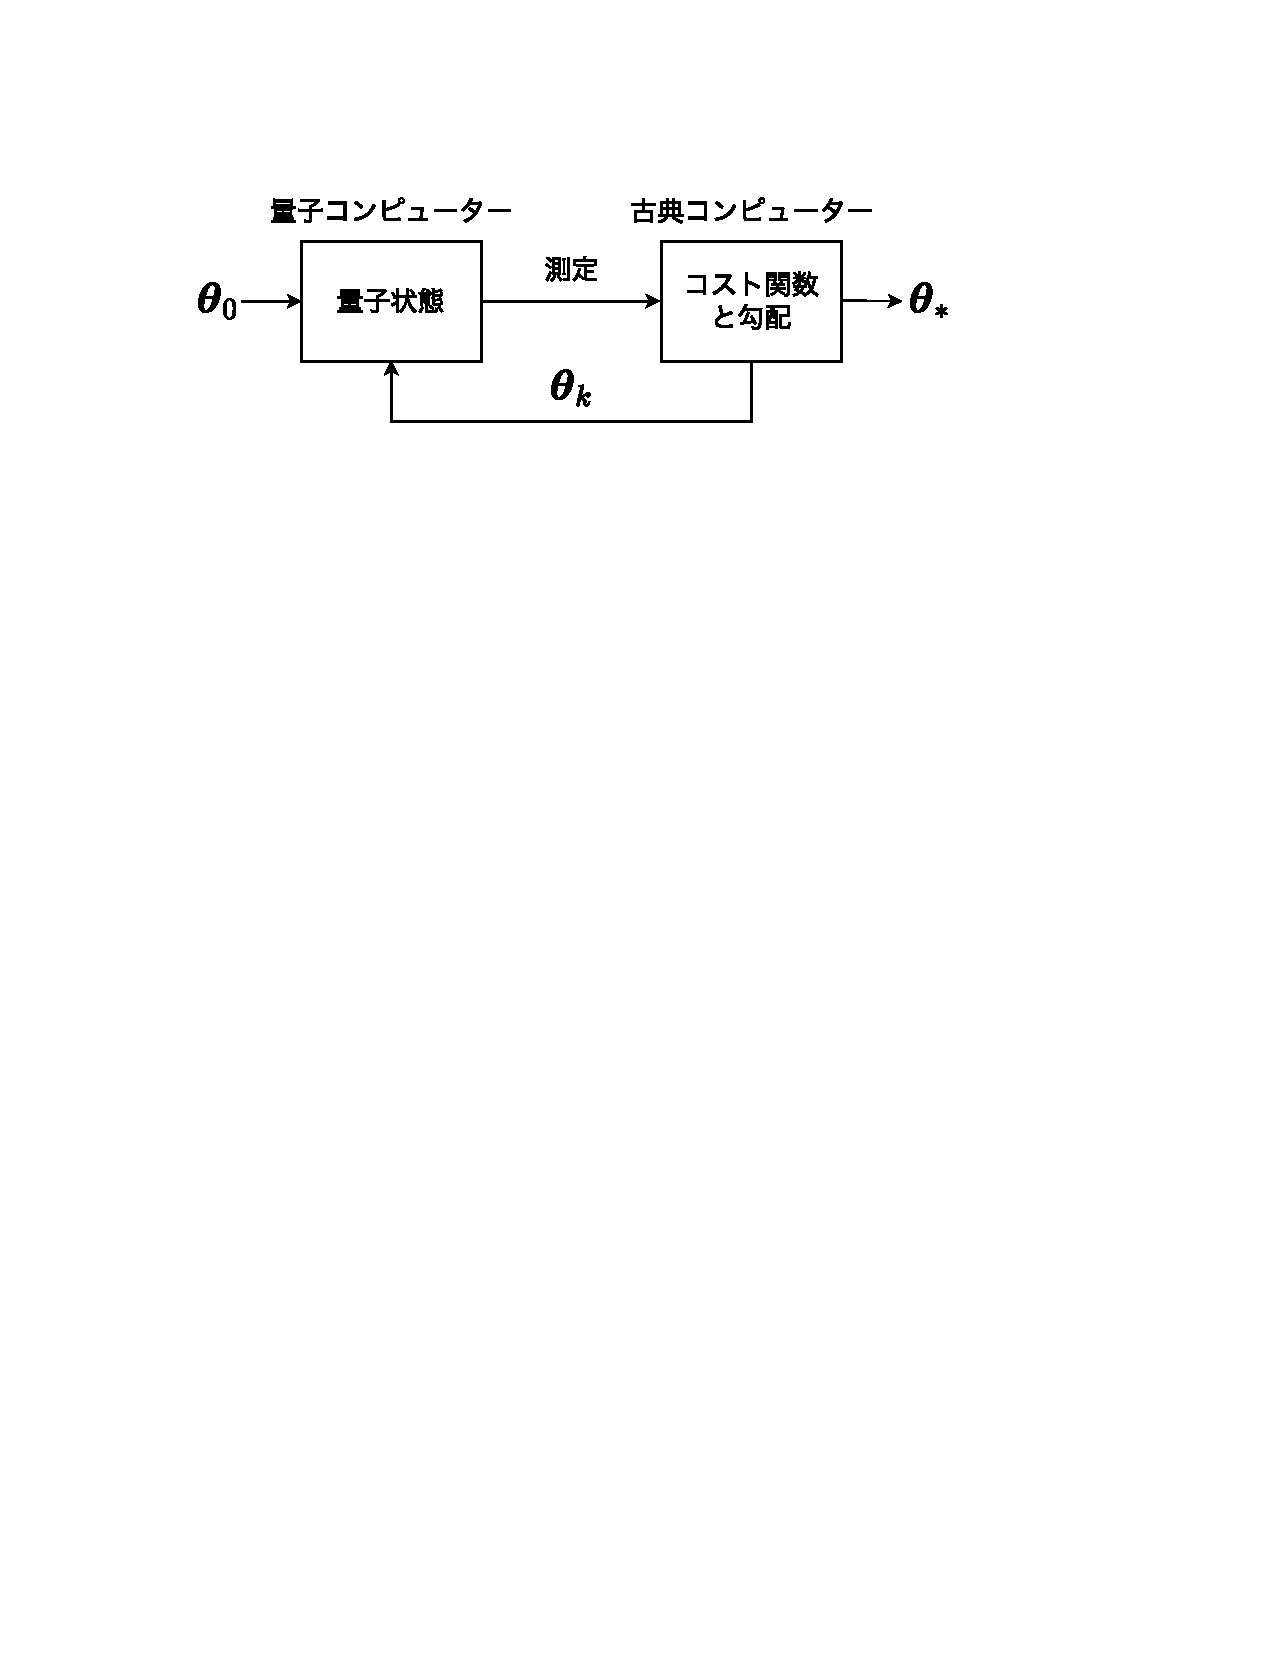
\includegraphics[width=11cm]{vqa-flow.pdf}
\end{frame}







\subsection{量子機械学習}
\begin{frame}{量子機械学習}
    ここでは、変分量子回路を用いた機械学習を\textcolor{blue}{量子機械学習}(Quantum Machine Learning)と呼ぶ。教師あり量子機械学習ではデータセット$\{\bx_i,\by_i\}_i$の\textcolor{blue}{入力回路}が必要となる。
    
    \begin{center}
        {\large\colorbox{blue!40}{\makebox[28em]{教師あり学習のコスト関数(量子回路学習モデル{\small[\href{http://arxiv.org/abs/1803.00745}{Mitarai2018}]})}}}
    \end{center}
    \begin{columns}
        \begin{column}{0.5\textwidth}
            \centering
            試行関数\\
            $\ket{\phi(\bx_i,\bth)} := V(\bth)U(\bx_i)\ket{0}^{\otimes n}$\\
            \vspace*{10pt}
            予測ラベル\\
            $\ell_{i}(\bth) := \expval{O}{\phi(\bx_i,\bth)}$\\
            \vspace*{10pt}
            コスト関数\\
            $\calL(\bth) := \frac1N\sum_{i=1}^N f(y_i,\ell_{i}(\bth))$
        \end{column}

        \begin{column}{0.5\textwidth}
            \begin{center}
                \begin{tikzpicture}
                    \node[scale=1]{
                    \begin{quantikz}
                        \lstick{$\ket{0}$} & \gate[3,bundle={2}][1cm]{U(\bx_i)} & \gate[3,bundle={2}][1cm]{V(\bth)} & \meter{} \\
                        \lstick{$\vdots$}\,\,& & & \,\,\vdots\qwbundle[alternate]{}  \\
                        \lstick{$\ket{0}$} & & \qw & \meter{} \\
                    \end{quantikz}};
                \end{tikzpicture}
            \end{center}
            \vspace*{-30pt}
            \hspace*{55pt}  ↑    ↑\\
            \hspace*{55pt}  入力回路 学習回路\\
            % \vspace*{10pt}
            % $f$ は二乗誤差などの関数。
        \end{column}
    \end{columns}
\end{frame}





\subsection{バレンプラトー (BP)}
\begin{frame}{バレンプラトー (Barren Plateau, BP)}
    \begin{columns}
        \vspace*{-50pt}
        \begin{column}{0.65\textwidth}
            \begin{center}
                {\large\colorbox{blue!40}{\makebox[17em]{バレンプラトー {\small[\href{http://arxiv.org/abs/1803.11173}{Mcclean2018}]}}}}
            \end{center}
            \vspace*{-10pt}
            \begin{definition}
                $\calL(\bs{\theta})$:コスト関数、$V(\bs{\theta})$:学習回路、$n$:量子ビット数
                $$\E_{V(\bth)}\left[\frac{\pd \calL(\bth)}{\pd \theta_\nu}\right] = 0, \,\,\Var_{V(\bth)}\left[\frac{\pd \calL(\bth)}{\pd \theta_\nu}\right] \in \calO(2^{-\alpha n}), \,\,\alpha > 0 $$
            \end{definition}
            勾配消失 → コスト関数の測定回数が指数関数的に増加\\
             \textcolor{blue}{勾配の分散のスケーリング}が計算量に影響
            \begin{center}
                \begin{tikzpicture}[scale=0.8]
                    \def\a{1}
                    \def\b{0.8}
                    \def\c{0.1}
                    \def\d{2.2}
                    \draw [domain=0:4,smooth] plot (\x,{-2*\b^2/(\b^2 + (\x-2)^2) + \d});
                    \draw [domain=5:9,smooth] plot (\x,{-2*\c^2/(\c^2 + (\x-7)^2) + \d});
                    \draw [->,thick] (0,2.7) -- (9.5,2.7) node [right]{$n$};
                    \draw [->] (0,0) -- (4,0) node [right]{$\theta_\nu$};
                    \draw [->] (5,0) -- (9,0) node [right]{$\theta_\nu$};
                \end{tikzpicture}
            \end{center}
        \end{column}

        \begin{column}{0.35\textwidth}
            {\large 原因}
            \begin{itemize}
                \item 学習回路の深さ
                \item オブザーバブルの局所性
                \item ノイズ
                \item \textcolor{blue}{データの入力}
            \end{itemize}

            \begin{figure}
                \centering
                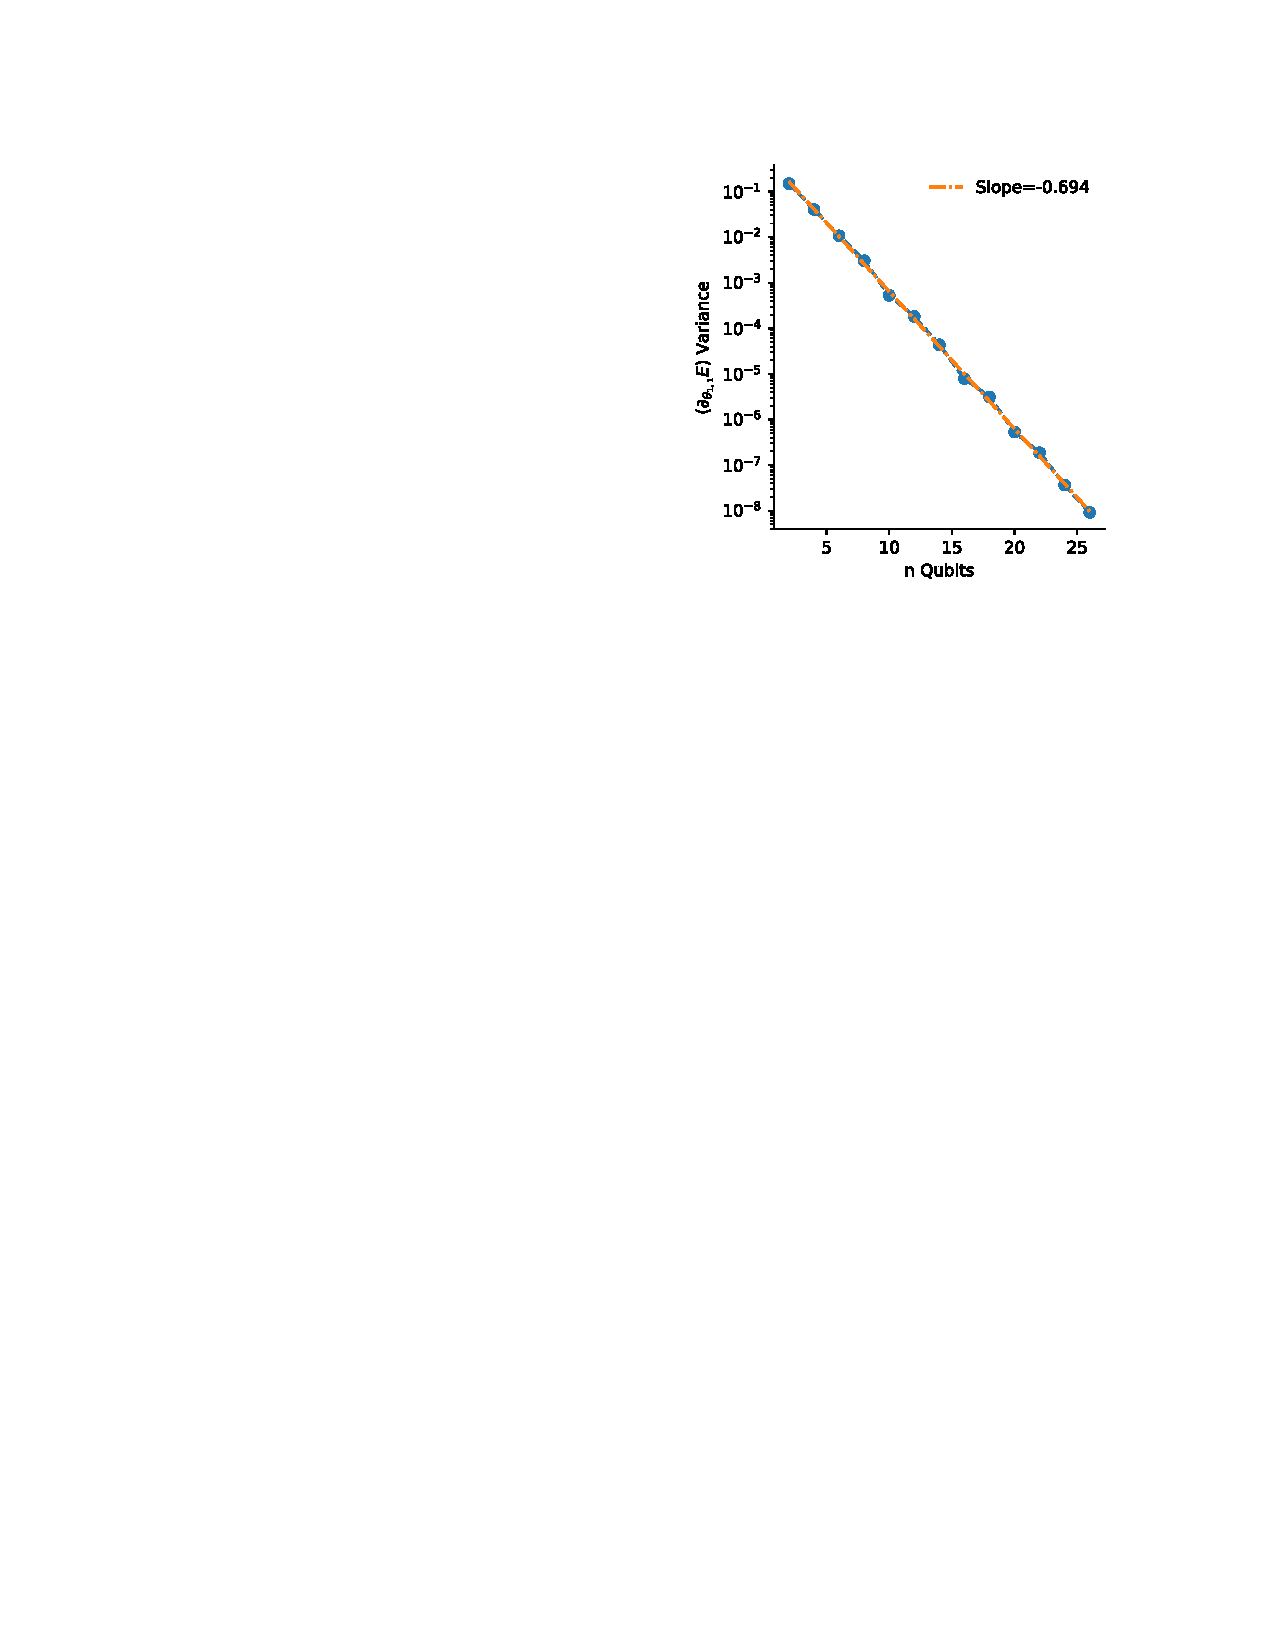
\includegraphics[height=4cm,width=4cm]{bp-var.pdf}
                \vspace*{-5pt}
                \caption{コスト関数の勾配の分散}
            \end{figure}
        \end{column}
    \end{columns}
\end{frame}




\section{研究概要}
\begin{frame}{研究概要}

    \vspace*{-20pt}
    \begin{center}
        {\large\colorbox{blue!40}{\makebox[15em]{研究背景}}}
    \end{center}
    \begin{center}
        \begin{minipage}{0.8\textwidth}
            \begin{itemize}
                \item 変分量子アルゴリズムによって機械学習を効率化したい
                \item しかし、バレンプラトー(勾配消失)が起きうる
                \item また、データの入力が与える影響は詳しく調べられていない
            \end{itemize}
        \end{minipage}
    \end{center}

    \begin{center}
        {\large\colorbox{blue!40}{\makebox[15em]{研究目的と方針}}}
    \end{center}

    目的:データ入力によってバレンプラトーが生じないようにする\\
    \vspace*{5pt}
    方針:\circled{1}データ入力とコスト関数の勾配の分散の関係を解析する(新規性)\\\hspace*{46pt}具体的には、コスト関数の勾配の分散の上界と下界を導出する。\\
    \vspace*{5pt}
    \hspace*{29pt}\circled{2}勾配の分散のスケーリングが誤差関数の形に依存しないことを数値検証
\end{frame}



\section{コスト関数の勾配の分散の上界}
\begin{frame}{コスト関数の勾配の分散の上界:設定}

    \centering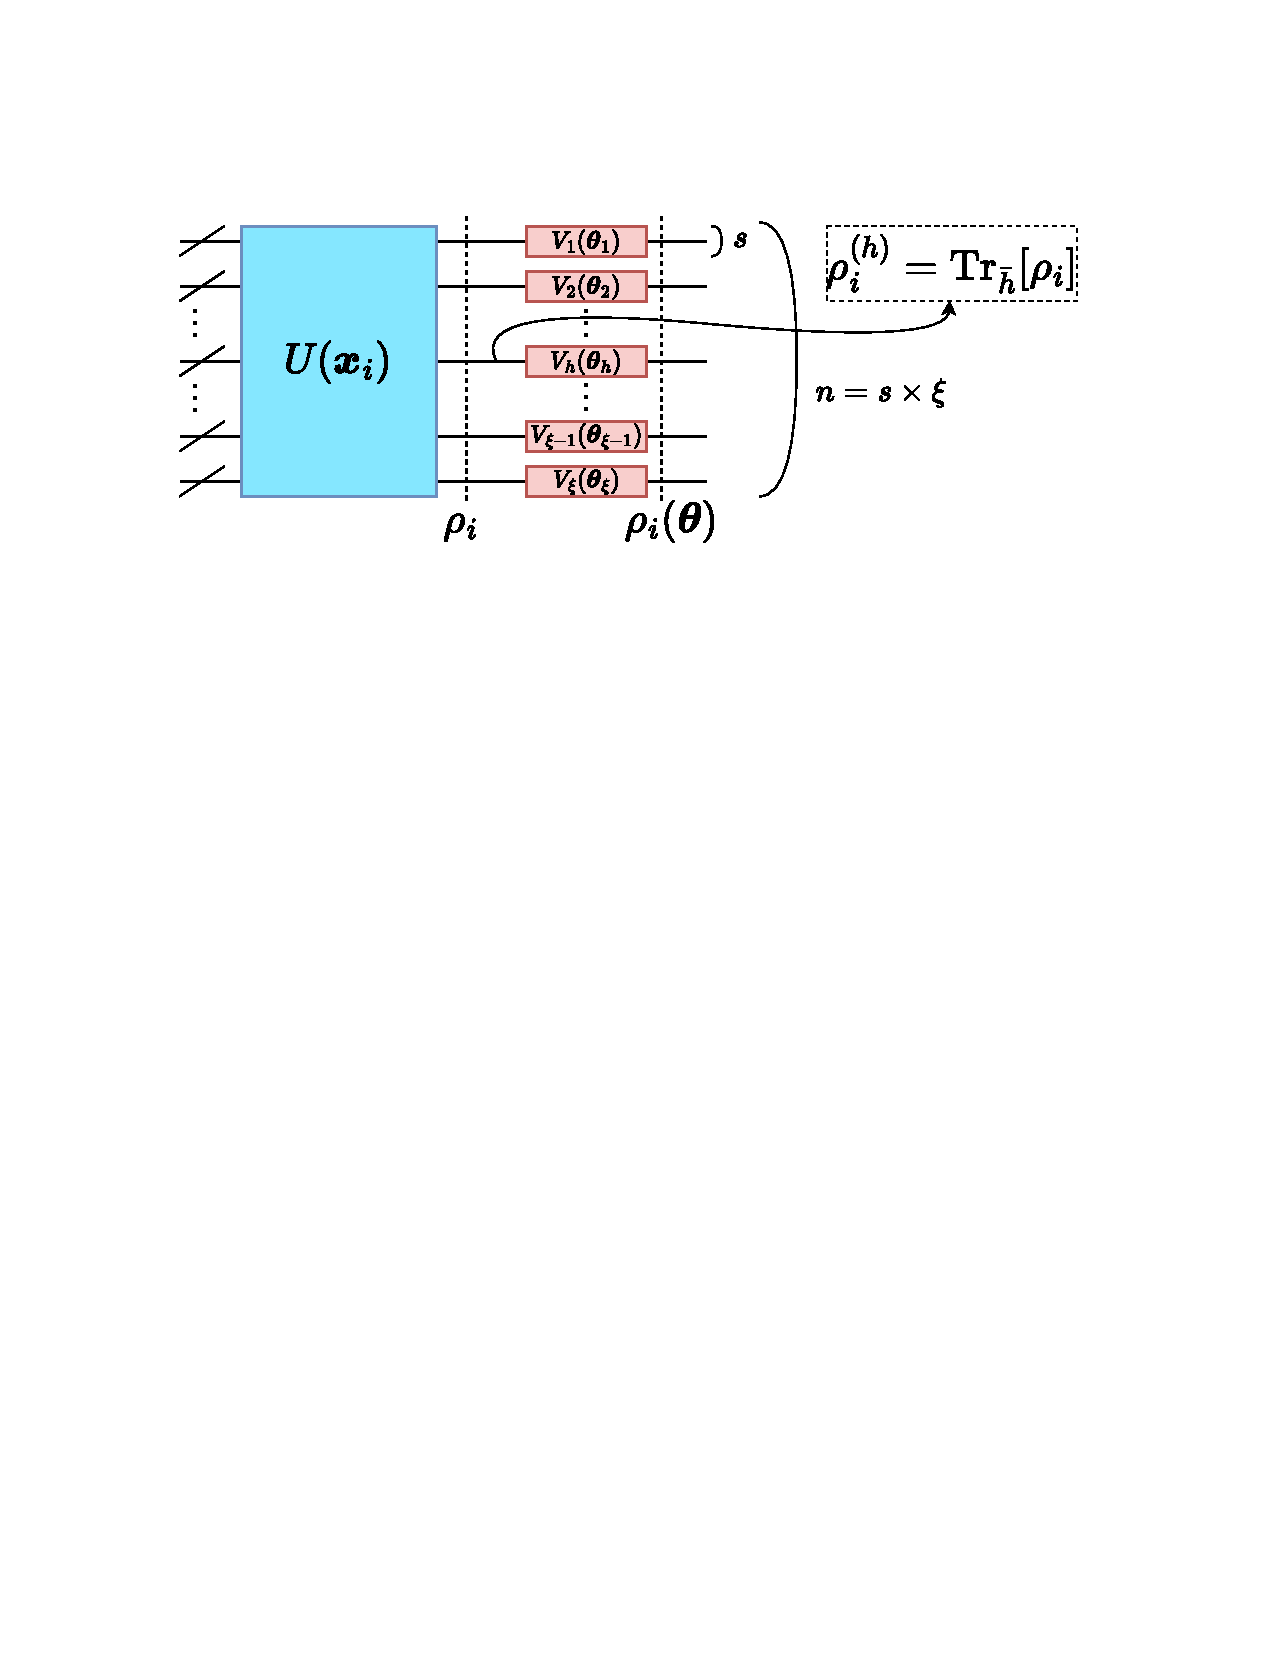
\includegraphics[width=12cm]{setting.pdf}
    $$
    \colorbox{orange!30}{$\ell_i(\bth)$} = \Tr[\rho_i(\bth)\,O_L] \in [0,1],
    \quad
    O_L=\frac1n \sum_{j=1}^{n}\dyad{0}_{j} \otimes \bbid_{\bar{j}}
    $$\\
    \vspace*{5pt}
    データ入力以外の要因でバレンプラトーが起きないように学習回路や $O_L$ を設定。
    
    % \begin{columns}
    %     \begin{column}{0.65\textwidth}
    %         \centering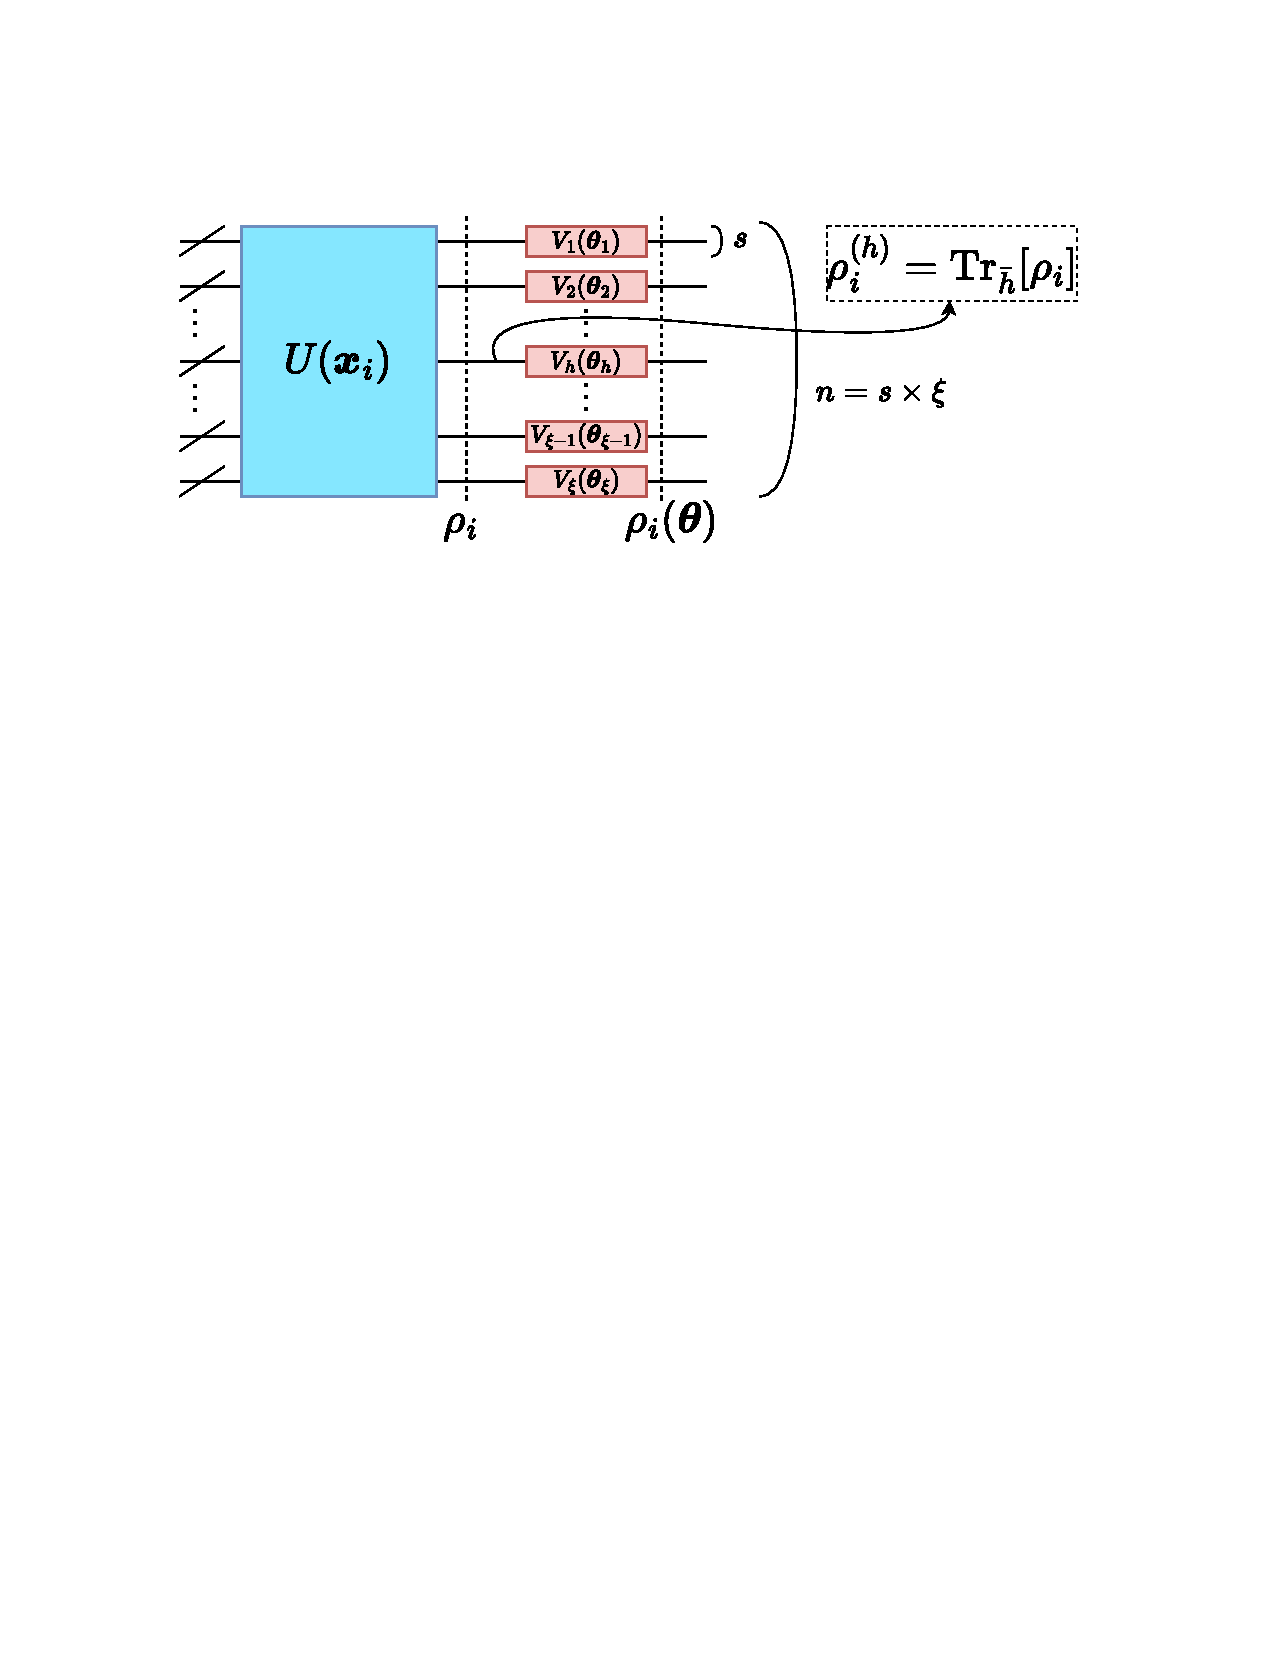
\includegraphics[width=8cm]{setting.pdf}
    %     \end{column}
    %     \vspace*{-20pt}
    %     \begin{column}{0.35\textwidth}
    %         $O_L=\frac1n \sum_{j=1}^{n}\dyad{0}_{j} \otimes \bbid_{\bar{j}}$.\\
    %         \vspace*{5pt}
    %         $\colorbox{orange!30}{$\ell_i(\bth)$} = \Tr[\rho_i(\bth)\,O_L] \in [0,1]$\\
    %         \vspace*{20pt}
    %         データ入力以外の要因\\
    %         によってBPが起きないように\\
    %         回路やコスト関数を設定。
    %     \end{column}
    % \end{columns}
    % \vspace*{-5pt}
    % 以下の定理\cite{cerezo2021cost}を解析に用いた。
    % \begin{theorem}
    %     \definecolor{myblue}{rgb}{0.2,0.4,0.8}
    %     $\theta_\nu$ は、上の図で$h$番目のブロックに含まれるパラメータとする。この時、$\Var_{V(\bth)}[\pd_{\theta_\nu}\ell_i(\bth)]$ は、\colorbox{myblue!20}{$\rho_i^{(h)}=\Tr_{\bar{h}}[\rho_i]$}と最大混合状態の間のHilbert Schmidt距離を用いて表すことができる。
    %     \vspace*{-10pt}
    %     \begin{align*}
    %         \Var_{V(\bth)}[\pd_{\theta_\nu} \colorbox{orange!30}{$\ell_i(\bth)$}] = r_{n,s}\times D_{\mathrm{HS}} ( \colorbox{myblue!20}{$\rho_i^{(h)}$} , \bbid/2^s ),
    %         \quad r_{n,s} \in O(1/n^2)
    %     \end{align*}
    % \end{theorem}
\end{frame}




\begin{frame}{コスト関数の勾配の分散の上界:結果}
    \vspace*{-15pt}
    $$y_i \in \{0,1\},\quad \colorbox{orange!30}{$\ell_i(\bth)$} := \Tr[\rho_i(\bth)\,O_L] \in [0,1],\quad
    \colorbox{green!30}{$\calL(\bth)$} := \frac1N\sum_{i=1}^N f(y_i, \colorbox{orange!30}{$\ell_i(\bth)$})$$
    \vspace*{-5pt}
    先行研究{\small[\href{https://arxiv.org/abs/2110.14753v1}{Thanasilp2021}]}を基に、新たな上界を与えた。

    \begin{theorem}
        量子機械学習において、前述の量子回路を用い、パラメータをランダムにサンプリングしたとき($V_j(\bth_j)$ がユニタリ $2$--デザイン)、コスト関数の勾配の分散の上界は次のように与えられる。ただし、$\bbU := \{U(\bs{x})|\,\bs{x}\in \calX\}$
        \vspace*{-10pt}
        \begin{align*}
            \Var_{V(\bth)}[\pd_{\theta_\nu} \colorbox{green!30}{$\calL(\bth)$}] \;\;
            \leq\;\;
            A_f \times r_{n,s} \times \bar{D}_{\mathrm{HS}}^s \;\;
            \leq\;\;
            A_f \times r_{n,s} \times \qty(\frac{2^s-2^{-s}}{2^n+1} + \epsilon_{\bbU})
        \end{align*}
    \end{theorem}

    \begin{itemize}
        \item $A_f$ は二乗誤差などの誤差関数 $f$ に依る項
        \item $r_{n,s}$ は測定するオブザーバブルに依る項
        \item $\bar{D}_{\mathrm{HS}}^s := \int_{\bbU}dU D_{\mathrm{HS}} ( \rho^{(h)} ,\, \bbid/2^s )$ はデータ入力に依る項
        \item $\epsilon_{\bbU}$ は入力回路の表現能力の指標であり、表現能力が高いほどこの値は小さい。
    \end{itemize}

    $\epsilon_{\bbU}$ が $0$にならない仮定の下、
    データ入力に依る項 $\bar{D}_{\mathrm{HS}}^s$ が指数的に落ちない条件を調べた。
\end{frame}





\newcommand{\bgbs}[1]{\gate[wires=2,style={fill=cyan!50}][1cm][0.1cm]{}\slice{#1}}
\newcommand{\bgb}{\gate[wires=2,style={fill=cyan!50}][1cm][0.1cm]{}}
\newcommand{\agb}{\gate[wires=1,style={fill=red!50}][1cm][0.5cm]{}}
\begin{frame}{コスト関数の勾配の分散の上界:具体的な入力回路}
    入力回路$U(\bx)$に次の Alternating Layered Ansatz (ALT) を仮定して、$\bar{D}_{\mathrm{HS}}^{s=1}$ を解析計算${}^\text{*}$
    \begin{figure}[H]
        \centering
        \begin{tikzpicture}
            \node[scale=0.7]{
            \begin{quantikz}
                \qw &\bgbs{1}& \qw     &\bgbs{3}& \qw     & \bgbs{5}& \agb & \qw\\[-0.3cm]
                \qw & \qw    & \bgbs{2}& \qw    & \bgbs{4}& \qw     & \agb & \qw\\[-0.3cm]
                \qw & \bgb   & \qw     & \bgb   & \qw     & \bgb    & \agb & \qw\\[-0.3cm]
                \qw & \qw    & \bgb    & \qw    & \bgb    & \qw     & \agb & \qw\\[-0.3cm]
                \qw & \bgb   & \qw     & \bgb   & \qw     & \bgb    & \agb & \qw\\[-0.3cm]
                \qw & \qw    & \bgb    & \qw    & \bgb    & \qw     & \agb & \qw\\[-0.3cm]
                \qw & \bgb   & \qw     & \bgb   & \qw     & \bgb    & \agb & \qw\\[-0.3cm]
                \qw & \qw    & \qw     & \qw    & \qw     & \qw     & \agb & \qw
            \end{quantikz}
            };
        \end{tikzpicture}
        \caption{青は入力回路、赤は学習回路}
        \label{fig:alt-tpa-structure}
    \end{figure}
    \vspace*{-5pt}
    学習回路としての ALT の BP への影響は先行研究{\small[\href{http://www.nature.com/articles/s41467-021-21728-w}{Cerezo2021}]}で調べられた。\\
    \begin{scriptsize}
        (*青いブロックがユニタリ $2$--デザインとして、Random Tensor Network Integrator (RTNI) [\href{http://arxiv.org/abs/1902.08539}{Fukuda2019}]を用いて計算)
    \end{scriptsize}
\end{frame}





\begin{frame}{コスト関数の勾配の分散とその上界の比較}\label{qml-var-alt}
    \begin{columns}
        \begin{column}{0.5\textwidth}
            \centering $\Var_{V(\bth)}[\pd_{\theta_\nu} \calL(\bth)]$
            \vspace{-10pt}
            \begin{figure}
                \centering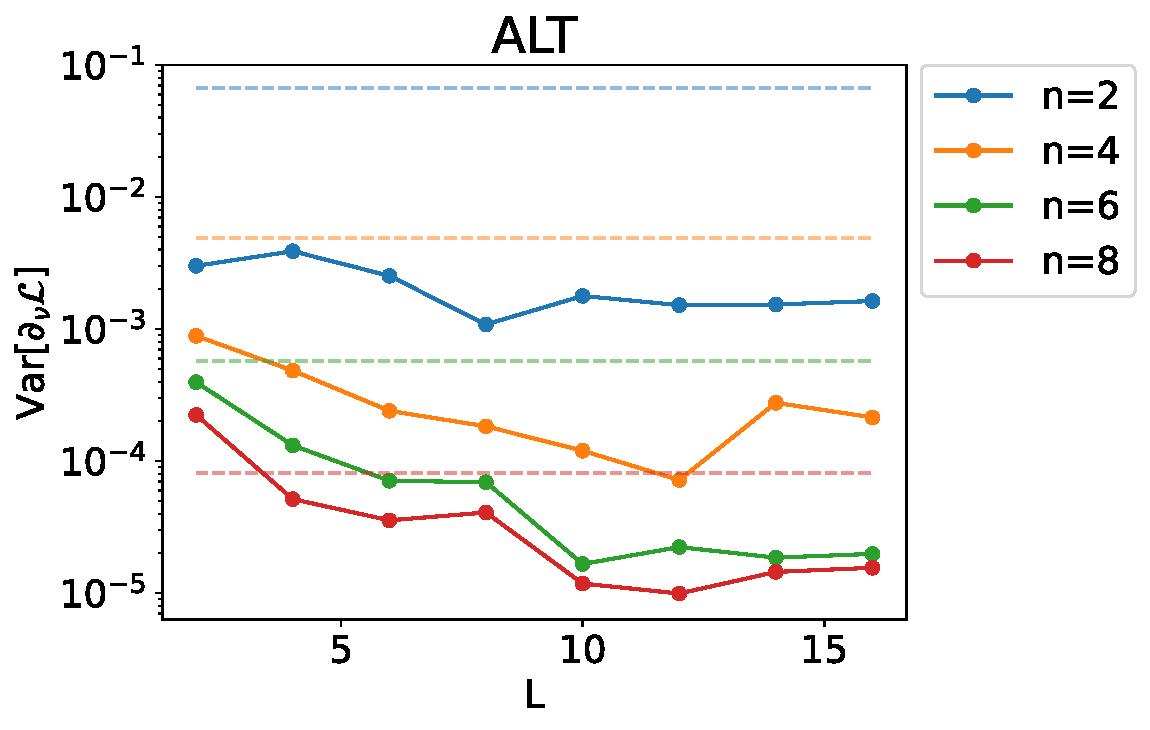
\includegraphics[width=7cm]{qml-var-alt.pdf}
            \end{figure}
        \end{column}
        \begin{column}{0.5\textwidth}
            \centering 上界($A_f \times r_{n,s} \times \bar{D}_{\mathrm{HS}}^{s=1}$)
            \vspace{-10pt}
            \begin{figure}
                \centering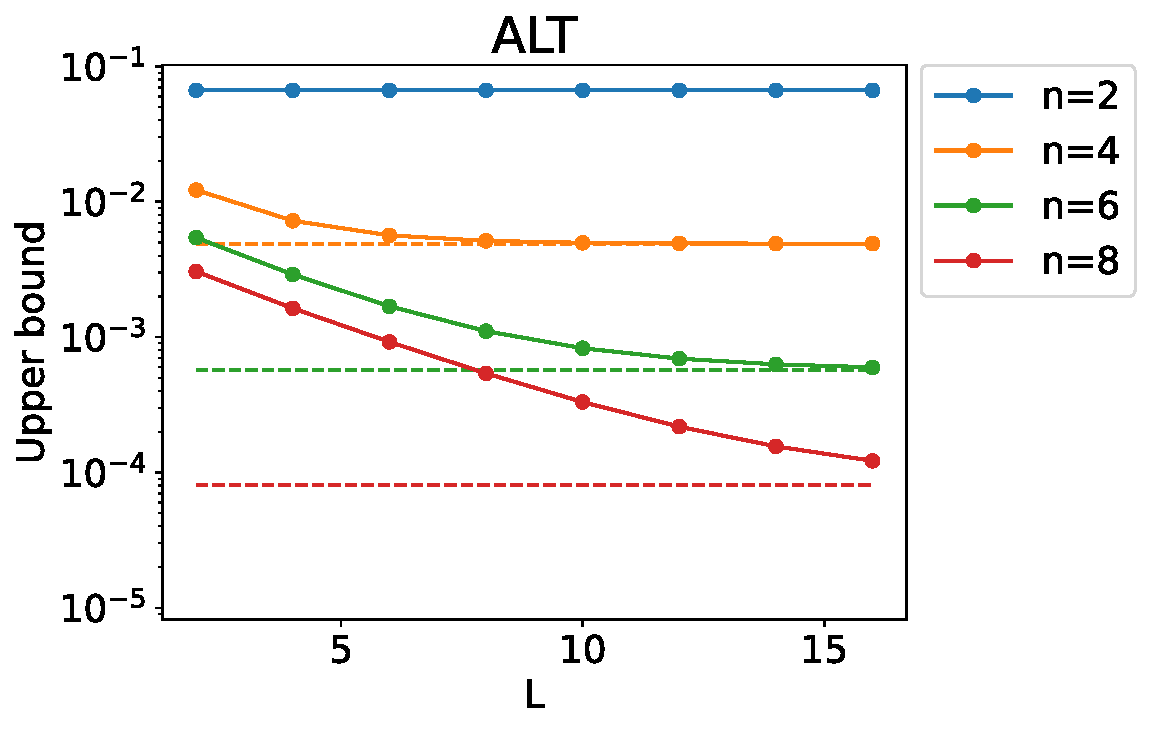
\includegraphics[width=7cm]{qml-var-bound-alt.pdf}
            \end{figure}
        \end{column}
    \end{columns}
    
    \vspace{-10pt}
    \begin{columns}
        \begin{column}{0.5\textwidth}
            \begin{figure}[H]
                \centering
                \begin{tikzpicture}
                    \node[scale=0.6]{
                        \begin{quantikz}
                            \qw & \gate[wires=2,style={fill=cyan!50}][1cm]{}& \qw\\
                            \qw & \qw                  & \qw
                        \end{quantikz}
                        \begin{quantikz}
                            {\LARGE \textbf{=}}
                        \end{quantikz}
                        \begin{quantikz}
                            \qw & \gate{R_x}&\gate{R_y}&\ctrl{1}& \qw\\
                            \qw & \gate{R_x}&\gate{R_y}&\targ{} & \qw
                        \end{quantikz}
                        };
                \end{tikzpicture}
            \end{figure}
            \begin{footnotesize}
                (アヤメのデータセットを用いてコスト関数を定義)\\
            \end{footnotesize}
        \end{column}
        \begin{column}{0.5\textwidth}
            \begin{figure}[H]
                \centering
                \begin{tikzpicture}
                    \node[scale=0.6]{
                        \begin{quantikz}
                            \qw & \gate[wires=2,style={fill=cyan!50}][1cm]{}& \qw\\
                            \qw & \qw                  & \qw
                        \end{quantikz}
                        \begin{quantikz}
                            {\LARGE \textbf{=}}
                        \end{quantikz}
                        \begin{quantikz}
                            \text{\LARGE ユニタリ 2--デザイン}
                        \end{quantikz}
                        };
                \end{tikzpicture}
            \end{figure}
            \begin{center}
                確かに上界の役割を果たしている
            \end{center}
        \end{column}
    \end{columns}
\end{frame}




\begin{frame}{層数の必要条件}
    上界が量子ビット数に対して指数関数的に落ちないための層数の設定\\
    \vspace*{10pt}
    \begin{columns}
        \begin{column}{0.65\textwidth}
            \begin{figure}
                \centering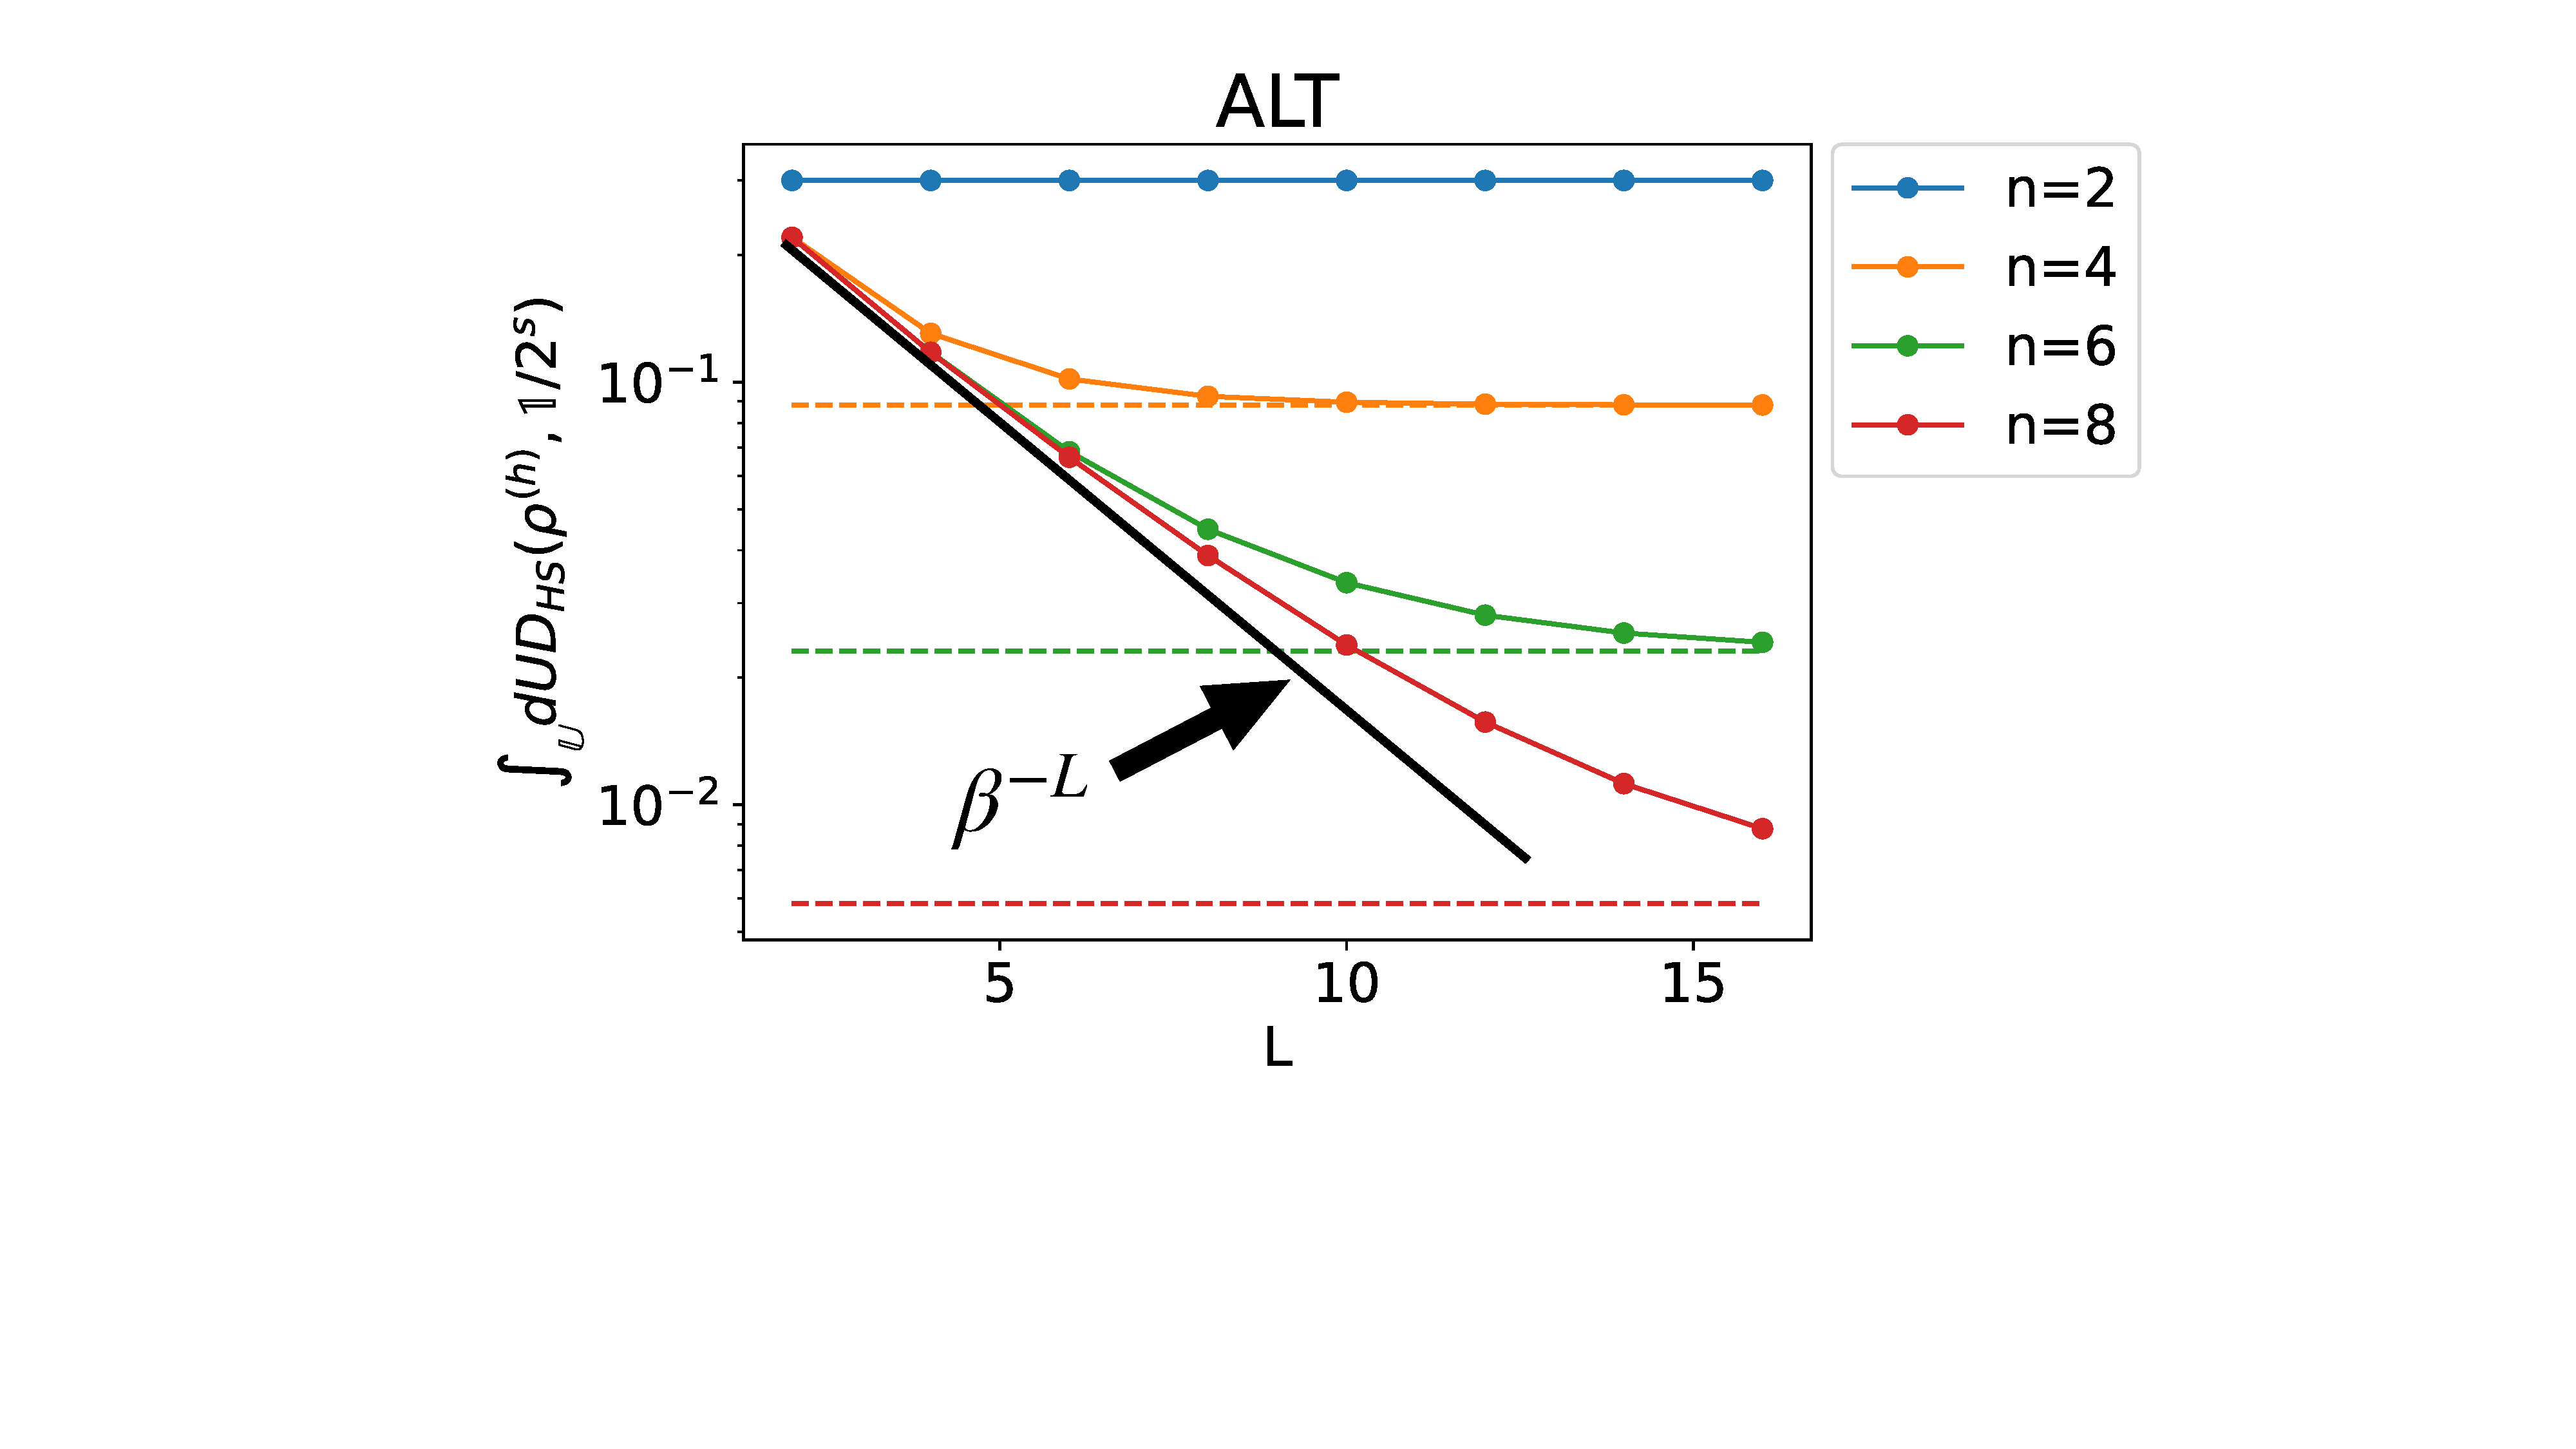
\includegraphics[width=8cm]{hsd-alt-analytical-with-line.pdf}
            \end{figure}
        \end{column}

        \begin{column}{0.35\textwidth}
            {\footnotesize($0<\alpha$, $n$: 量子ビット数)}\\
            \vspace*{2pt}
            $\bar{D}_{\mathrm{HS}}^s \propto e^{-\alpha n}$ → BP\\

            \vspace*{10pt}
            BPが起きない必要条件:\\
            {\footnotesize($0<\gamma,\;1<\beta$)}\\
            \vspace*{2pt}
            $n^{-\gamma} \leq \beta^{-L} \leq \bar{D}_{\mathrm{HS}}^s$\\
            \vspace*{2pt}
            \hspace*{5pt}$\;\Longrightarrow\;$\textcolor{blue}{$L \leq \frac{\gamma}{\log{\beta}}\log{n}$}\\

            \vspace*{10pt}
            (BP: バレンプラトー)
        \end{column}
    \end{columns}
\end{frame}



% \begin{frame}{上界のまとめ}
%     \begin{itemize}
%         \item コスト関数の勾配の分散の上界をデータ入力の観点から導出し、数値的にも検証を行った。
%         \item その結果、データ入力後の状態のエンタングルメントや入力回路の表現能力が大きいほど、コスト関数の勾配の分散の上界が小さくなり、バレンプラトーにつながることが明らかになった。
%         \item また、コスト関数の勾配の分散の上界が量子ビット数に対して指数関数的に落ちないための層数の必要条件を調べ、層数 $L$ が量子ビット数 $n$ に対して $L \order{\log{n}}$ でなければならないことを示した。
%     \end{itemize}
% \end{frame}



\section{コスト関数の勾配の分散の下界}

\newcommand{\bgate}[1]{\gate[wires=1,style={fill=cyan!50}][1cm][0.7cm]{\Large #1}}
\newcommand{\rgate}[1]{\gate[wires=4,style={fill=red!50}]{\Large #1}}
\begin{frame}{コスト関数の勾配の分散の下界:設定}
    \vspace*{-10pt}
    \begin{columns}
        \begin{column}{0.4\textwidth}
            \begin{footnotesize}
                (解析のため単純な入力回路を仮定)
            \end{footnotesize}
            \begin{itemize}
                \setlength{\itemsep}{10pt}
                \item 量子回路:\\$n = s\times\xi$ 量子ビット\\$R_y$ ゲートからなる入力回路
                \item コスト関数(2値分類):$\calL_{\mathrm{MAE}}(\bth) = \frac1N\sum_{i=1}^N |\ell_{i}(\bth) - y_i|$
                \item 入力データ:\\$\calX = \{\bs{x}\}$ (ラベル $0$)\\$\calZ = \{\bs{z}\}$ (ラベル $1$)\\$|\calX|:|\calZ| = p:q\;(p+q=1)$
                \item ガウス分布:$x_{j,d} \sim \calN(\mu_{x|j,d}, \sigma_{x|j,d}^2)$\\$z_{j,d} \sim \calN(\mu_{z|j,d}, \sigma_{z|j,d}^2)$
                \item 分散:$\sigma_{x|j,d},\, \sigma_{z|j,d} \leq \sigma_{\max}$
            \end{itemize}
        \end{column}
        \begin{column}{0.6\textwidth}
        \begin{figure}[H]
            \centering
            \begin{tikzpicture}
            \node[scale=0.5]{
                \begin{quantikz}
                    \lstick{$\ket{0}$} & \bgate{R_y(x_{1,1})}    & \bgate{R_y(x_{1,2})}    &\qw \ \ldots\ & \bgate{R_y(x_{1,L})}    &\rgate{V_1(\bth_1)}& \meter{} \\
                    \lstick{$\ket{0}$} & \bgate{R_y(x_{2,1})}    & \bgate{R_y(x_{2,2})}    &\qw \ \ldots\ & \bgate{R_y(x_{2,L})}    & \qw                     & \meter{} \\
                    \wave&&&&&&&&&\\
                    \lstick{$\ket{0}$} & \bgate{R_y(x_{s,1})}    & \bgate{R_y(x_{s,2})}    &\qw \ \ldots\ & \bgate{R_y(x_{s,L})}    & \qw                     & \meter{}\\
                    \lstick{$\ket{0}$} & \bgate{R_y(x_{s+1,1})}  & \bgate{R_y(x_{s+1,2})}  &\qw \ \ldots\ & \bgate{R_y(x_{s+1,L})}  &\rgate{V_2(\bth_2)}& \meter{} \\
                    \lstick{$\ket{0}$} & \bgate{R_y(x_{s+2,1})}  & \bgate{R_y(x_{s+2,2})}  &\qw \ \ldots\ & \bgate{R_y(x_{s+2,L})}  & \qw                     & \meter{} \\
                    \wave&&&&&&&&&\\
                    \lstick{$\ket{0}$} & \bgate{R_y(x_{2s,1})}   & \bgate{R_y(x_{2s,2})}   &\qw \ \ldots\ & \bgate{R_y(x_{2s,L})}   & \qw                     & \meter{}\\
                    \wave&&&&&&&&&\\
                    \lstick{$\ket{0}$} & \bgate{R_y(x_{n-s+1,1})}& \bgate{R_y(x_{n-s+1,2})}&\qw \ \ldots\ & \bgate{R_y(x_{n-s+1,L})}&\rgate{V_\xi(\bth_\xi)}& \meter{} \\
                    \lstick{$\ket{0}$} & \bgate{R_y(x_{n-s+2,1})}& \bgate{R_y(x_{n-s+2,2})}&\qw \ \ldots\ & \bgate{R_y(x_{n-s+2,L})}& \qw                     & \meter{} \\
                    \wave&&&&&&&&&\\
                    \lstick{$\ket{0}$} & \bgate{R_y(x_{n,1})}    & \bgate{R_y(x_{n,2})}    &\qw \ \ldots\ & \bgate{R_y(x_{n,L})}    & \qw                     & \meter{}
                \end{quantikz}};
            \end{tikzpicture}
            \caption{$L$ 層の $R_y$ ゲートからなる入力回路と\\$\xi$ 個の $s$量子ビットユニタリからなる $V_\xi(\bth_\xi)$ 学習回路}
            \label{fig:circuit-concentration-1}
        \end{figure}
        \end{column}
    \end{columns}
\end{frame}



\begin{frame}{コスト関数の勾配の分散の下界:結果}
    \begin{theorem}
        絶対誤差のコスト関数の勾配の分散は次のように下から抑えられる。
        \begin{align*}
            \frac{r_{n,s}}{2^s}\;
            \sum_{j=1}^s \qty(p\,e^{-\Sigma_{x|j}/2} - q\,e^{-\Sigma_{z|j}/2})^2
            \leq \Var_{V(\bth)}[\pd_\nu\calL_{\mathrm{MAE}}(\bth)]
            % \leq \frac{r_{n,s}}{2^s}\;\qty[\qty(1 + e^{-L\,\sigma_{\min}^2})^s - w^2]
        \end{align*}
        ただし、$r_{n,s} := \frac{s\,2^{3(s-1)}}{n^2(2^{2s}-1)^2}$, $\Sigma_{x|j} = \sum_{d=1}^L \sigma_{x|j,d}^2$, $\Sigma_{z|j} = \sum_{d=1}^L \sigma_{z|j,d}^2$
    \end{theorem}
    
    $|\calX|:|\calZ| = 1:1 \iff p = q = 1/2$ のとき、分散の下界は
    
    \begin{center}
        $
        \frac{r_{n,s}}{2^{s+2}}\;
        \sum_{j=1}^s
        \qty(e^{-\Sigma_{x|j}/2}- e^{-\Sigma_{z|j}/2})^2
        \leq \Var_{V(\bth)}[\pd_\nu\calL_{\mathrm{MAE}}(\bth)]
        $
    \end{center}

    \begin{itemize}
        \item 下界において分散に依存する $e^{-\Sigma_{x|j}/2},\,e^{-\Sigma_{z|j}/2}$ の差が重要
        \item しかし、$e^{-\Sigma_{x|j}/2},\,e^{-\Sigma_{z|j}/2}$ は層数に関して指数関数的に小さくなる
        \item すべての $j$ に対し $e^{-\Sigma_{x|j}/2} = e^{-\Sigma_{z|j}/2}$ である場合、下界は $0$ となる
    \end{itemize}
\end{frame}




\begin{frame}{コスト関数の勾配の分散の下界:結果}
    \begin{theorem}
        絶対誤差のコスト関数の勾配の分散は次のように下から抑えられる。
        \begin{align*}
            \frac{r_{n,s}}{2^s}\;
            \sum_{j=1}^s \qty(p\,e^{-\Sigma_{x|j}/2} - q\,e^{-\Sigma_{z|j}/2})^2
            \leq \Var_{V(\bth)}[\pd_\nu\calL_{\mathrm{MAE}}(\bth)]
            % \leq \frac{r_{n,s}}{2^s}\;\qty[\qty(1 + e^{-L\,\sigma_{\min}^2})^s - w^2]
        \end{align*}
        ただし、$r_{n,s} := \frac{s\,2^{3(s-1)}}{n^2(2^{2s}-1)^2}$, $\Sigma_{x|j} = \sum_{d=1}^L \sigma_{x|j,d}^2$, $\Sigma_{z|j} = \sum_{d=1}^L \sigma_{z|j,d}^2$
    \end{theorem}
    
    $|\calX|:|\calZ| = 1:0 \iff p = 1,\,q = 0$ のとき、分散の下界は
    
    \begin{center}
        $
            \frac{r_{n,s}s}{2^s}\; e^{-L\sigma_{\max}^2}
            \leq \frac{r_{n,s}}{2^s}\;\sum_{j=1}^s e^{-\Sigma_{x|j}}
            \leq \Var_{V(\bth)}[\pd_{\theta_\nu}\calL_{\mathrm{MAE}}(\bth)]
        $
    \end{center}

    \begin{itemize}
        \item $L\sigma_{\max}^2$ が小さいほど、分散の下界は大きくなる
        \item $s,\,L\sigma_{\max}^2 \in \order{\log{n}}$ である場合、分散の下界は $\order{1/\poly(n)}$ となる\\             → バレンプラトー回避の十分条件
    \end{itemize}
\end{frame}



\section{誤差関数の形とコスト関数の勾配の分散}
\begin{frame}{誤差関数の形とコスト関数の勾配の分散}
    誤差関数の形はコスト関数の勾配の分散のスケーリングにどのように影響するか?
    \begin{footnotesize}
        \begin{align*}
            \calL_{\mathrm{MAE}}(\bth) &= \frac1N\sum_{i=1}^N \abs{\ell_i(\bth) - y_i} \\
            \calL_{\mathrm{MSE}}(\bth) &= \frac1N\sum_{i=1}^N \qty(\ell_i(\bth) - y_i)^2 \\
            \calL_{\mathrm{LOG}}(\bth) &= \frac1N\sum_{i=1}^N [-y_i \log{\ell_i(\bth)} - (1-y_i)\log{(1-\ell_i(\bth))}] \\
        \end{align*}
        \vspace{-25pt}
        \begin{alignat*}{2}
            \implies
            \pd_{\theta_\nu} \calL_{\mathrm{MAE}}(\bth) &= \frac1N\sum_{i=1}^N &\sgn(\ell_i(\bth) - y_i) \cdot\pd_{\theta_\nu} \ell_i(\bth) \\
            \pd_{\theta_\nu} \calL_{\mathrm{MSE}}(\bth) &= \frac1N\sum_{i=1}^N 2|\ell_i(\bth) - y_i| &\sgn(\ell_i(\bth) - y_i)\cdot\pd_{\theta_\nu} \ell_i(\bth) \\
            \pd_{\theta_\nu} \calL_{\mathrm{LOG}}(\bth) &= \frac1N\sum_{i=1}^N \frac{1}{1 - |\ell_i(\bth) - y_i|} &\sgn(\ell_i(\bth) - y_i) \cdot\pd_{\theta_\nu} \ell_i(\bth) 
        \end{alignat*}
    \end{footnotesize}
    \begin{center}
        ただし、$y_i \in \{0,1\}$, $\quad \ell_i(\bth) = \Tr[\rho_i(\bth)\,O_L] \in [0,1]$,   $\quad (O_L = \frac1n \sum_{j=1}^{n}\dyad{0}_{j} \otimes \bbid_{\bar{j}})$
    \end{center}
\end{frame}




\begin{frame}{誤差関数の形とコスト関数の勾配の分散}
    学習回路がユニタリ $2$--デザインであると仮定した場合の $\ell_i(\bth)$ の平均と分散:
    \begin{align*}
        \E_{\calU(d)}[\ell_i(\bth)]  &= \frac12\\
        \Var_{\calU(d)}[\ell_i(\bth)]&= \frac{1}{4n(2^n+1)}
    \end{align*}
    そこで、すべての $i$ について $\ell_i(\bth) \sim \frac12 \iff |\ell_i(\bth) - y_i| \sim \frac12$ と仮定すると、
    \begin{align*}
        \pd_{\theta_\nu} \calL_{\mathrm{MSE}}(\bth) \sim \pd_{\theta_\nu} \calL_{\mathrm{MAE}}(\bth),\quad
        \pd_{\theta_\nu} \calL_{\mathrm{LOG}}(\bth) \sim 2\,\pd_{\theta_\nu} \calL_{\mathrm{MAE}}(\bth)
    \end{align*}
    となる。したがって、二乗誤差と絶対誤差、交差エントロピー誤差と絶対誤差の勾配の分散の比は次のように近似される。
    \begin{align*}
        \implies
        \Var_{\calU(d)}[\pd_{\theta_\nu}\calL_{\mathrm{MSE}}(\bth)]\,&/\,\Var_{\calU(d)}[\pd_{\theta_\nu}\calL_{\mathrm{MAE}}(\bth)] \sim 1\\
        \Var_{\calU(d)}[\pd_{\theta_\nu}\calL_{\mathrm{LOG}}(\bth)]\,&/\,\Var_{\calU(d)}[\pd_{\theta_\nu}\calL_{\mathrm{MAE}}(\bth)] \sim 4
    \end{align*}
    学習回路が深い場合、誤差関数によらず勾配の分散のスケーリングは同程度と推測される。
\end{frame}




\newcommand{\rgbt}{\gate[wires=2,style={fill=red!50}][1cm][0.1cm]{}}
\newcommand{\bgbo}{\gate[wires=1,style={fill=cyan!50}][1cm][0.5cm]{}}
\newcommand{\bgbog}{\gate[wires=1,style={fill=cyan!50}][1cm][0.5cm]{}\gategroup[8,steps=4,style={dashed, rounded corners, fill=cyan!20, inner xsep=1pt},background,label style={label position=below,anchor=north,yshift=-0.2cm}]{{\Large Shallow}}}
\newcommand{\gpd}{\ghost{H}\gategroup[8,steps=11,style={dashed, rounded corners, fill=red!20, inner xsep=3pt, inner ysep=21pt},background,label style={label position=below,anchor=north,yshift=-0.2cm}]{{\Large Deep}}}
\begin{frame}{誤差関数の形とコスト関数の勾配の分散:具体的な回路}
    学習回路に ALT を仮定して、その層数 $L_{\text{red}}$ を変化させたときのコスト関数の勾配の分散の比を調べる。(青は入力回路、赤は学習回路)
    \begin{figure}[H]
        \centering
        \begin{tikzpicture}
            \node[scale=0.65]{
            \begin{quantikz}
                \gpd     & \bgbog& \bgbo & \bgbo &\rgbt & \qw  &\rgbt & \qw  &\qw\ \ldots\ &\rgbt & \qw\\[-0.3cm]
                \ghost{H}& \bgbo & \bgbo & \bgbo & \qw  & \rgbt& \qw  & \rgbt&\qw\ \ldots\ & \qw  & \qw\\[-0.3cm]
                \ghost{H}& \bgbo & \bgbo & \bgbo & \rgbt& \qw  & \rgbt& \qw  &\qw\ \ldots\ & \rgbt& \qw\\[-0.3cm]
                \ghost{H}& \bgbo & \bgbo & \bgbo & \qw  & \rgbt& \qw  & \rgbt&\qw\ \ldots\ & \qw  & \qw\\[-0.3cm]
                \ghost{H}& \bgbo & \bgbo & \bgbo & \rgbt& \qw  & \rgbt& \qw  &\qw\ \ldots\ & \rgbt& \qw\\[-0.3cm]
                \ghost{H}& \bgbo & \bgbo & \bgbo & \qw  & \rgbt& \qw  & \rgbt&\qw\ \ldots\ & \qw  & \qw\\[-0.3cm]
                \ghost{H}& \bgbo & \bgbo & \bgbo & \rgbt& \qw  & \rgbt& \qw  &\qw\ \ldots\ & \rgbt& \qw\\[-0.3cm]
                \ghost{H}& \bgbo & \bgbo & \bgbo & \qw  & \qw  & \qw  & \qw  &\qw\ \ldots\ & \qw  & \qw
            \end{quantikz}
            };
        \end{tikzpicture}
    \end{figure}
    
    \vspace{-27pt}
    \begin{columns}
        \begin{column}{0.5\textwidth}
            \begin{figure}[H]
                \centering
                \begin{tikzpicture}
                    \node[scale=0.8]{
                        \begin{quantikz}
                            \qw & \gate[wires=1,style={fill=cyan!50}][1cm][0.7cm]{}& \qw
                        \end{quantikz}
                        \begin{quantikz}
                            {\LARGE \textbf{=}}
                        \end{quantikz}
                        \begin{quantikz}
                            \qw & \gate{R_x} &\gate{R_y} & \qw
                        \end{quantikz}
                        };
                \end{tikzpicture}
            \end{figure}
        \end{column}
        
        \begin{column}{0.5\textwidth}
            \begin{figure}[H]
                \centering
                \begin{tikzpicture}
                    \node[scale=0.7]{
                        \begin{quantikz}
                            \qw & \gate[wires=2,style={fill=red!50}][1cm]{}& \qw\\
                            \qw & \qw                  & \qw
                        \end{quantikz}
                        \begin{quantikz}
                            {\LARGE \textbf{=}}
                        \end{quantikz}
                        \begin{quantikz}
                            \qw & \gate{R_x}&\gate{R_y}&\ctrl{1}& \qw\\
                            \qw & \gate{R_x}&\gate{R_y}&\targ{} & \qw
                        \end{quantikz}
                        };
                \end{tikzpicture}
            \end{figure}
        \end{column}
    \end{columns}
\end{frame}





\begin{frame}{誤差関数の形とコスト関数の勾配の分散}
    \vspace{-10pt}
    \begin{columns}
        \begin{column}{0.5\textwidth}
            \begin{figure}
                \centering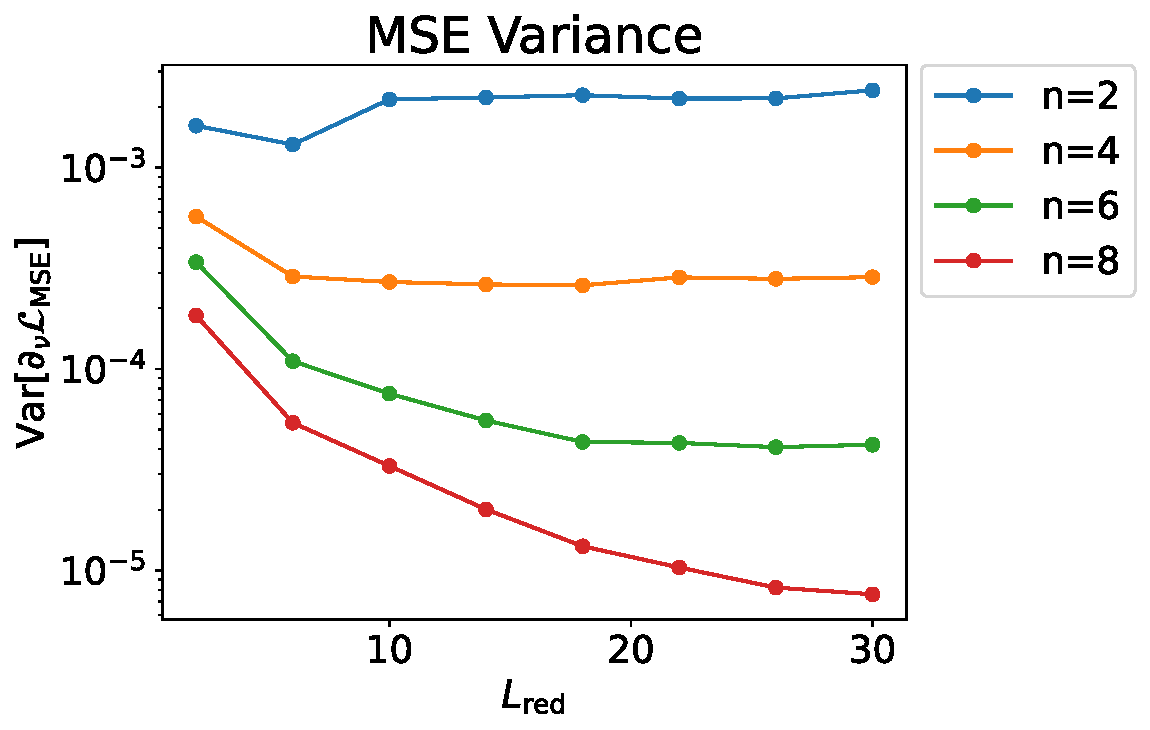
\includegraphics[width=6cm]{variance-mse_encoding3.pdf}
            \end{figure}
        \end{column}
        \begin{column}{0.5\textwidth}
            \begin{figure}
                \centering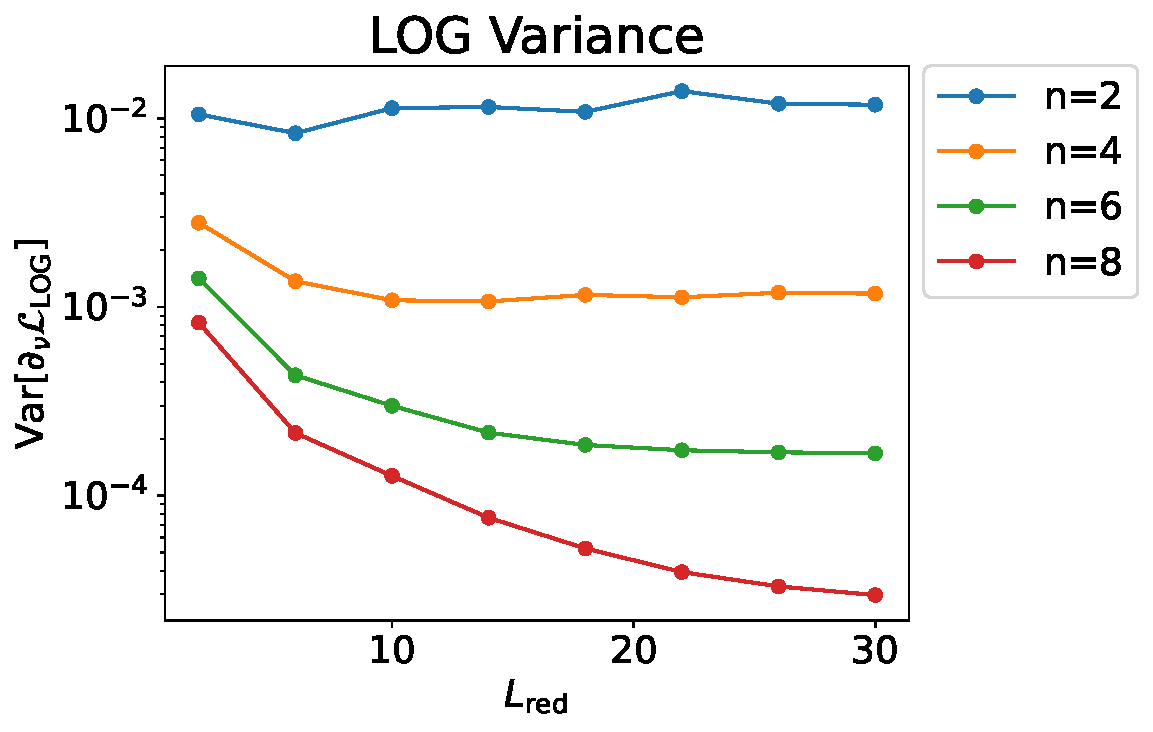
\includegraphics[width=6cm]{variance-log_encoding3.pdf}
            \end{figure}
        \end{column}
    \end{columns}
    \vspace{-15pt}
    \begin{figure}
        \centering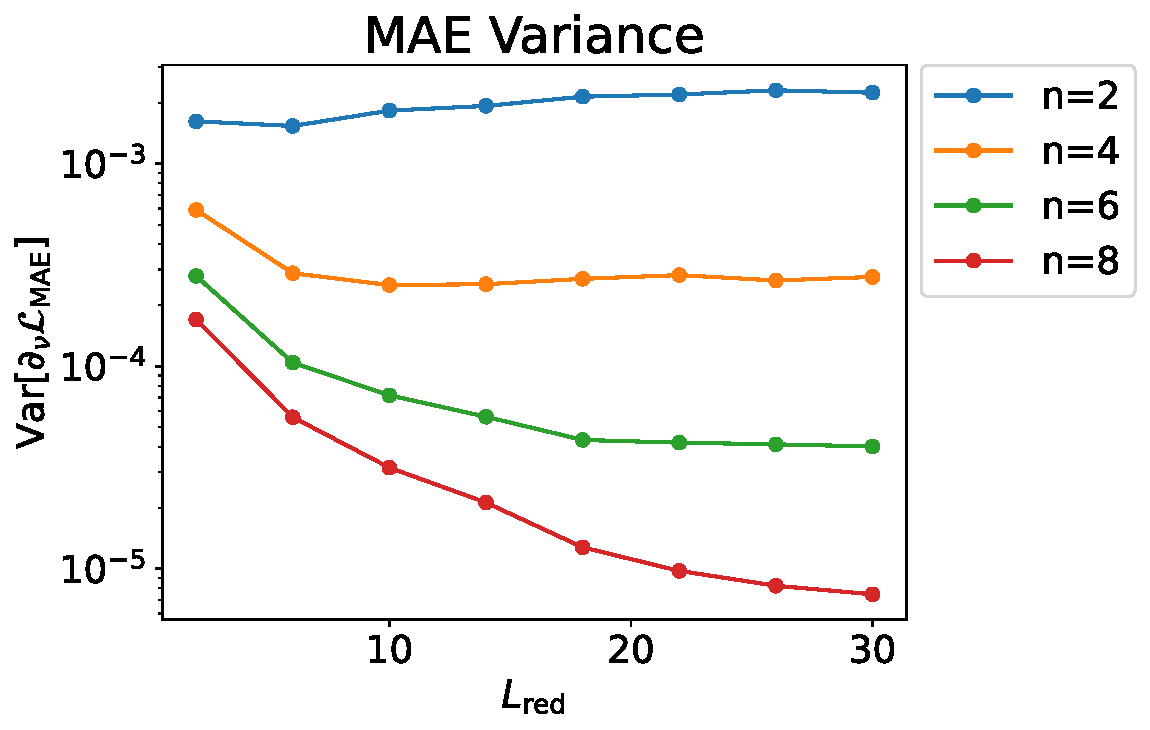
\includegraphics[width=6cm]{variance-mae_encoding3.pdf}
    \end{figure}
\end{frame}




\begin{frame}{誤差関数の形とコスト関数の勾配の分散}
    \begin{columns}
        \begin{column}{0.5\textwidth}
            \begin{small}
                \centering\hspace*{-10pt} $\Var_{V(\bth)}[\pd_{\theta_\nu}\calL_{\mathrm{MSE}}(\bth)]\,/\,\Var_{V(\bth)}[\pd_{\theta_\nu}\calL_{\mathrm{MAE}}(\bth)]$
            \end{small}
            \begin{figure}
                \centering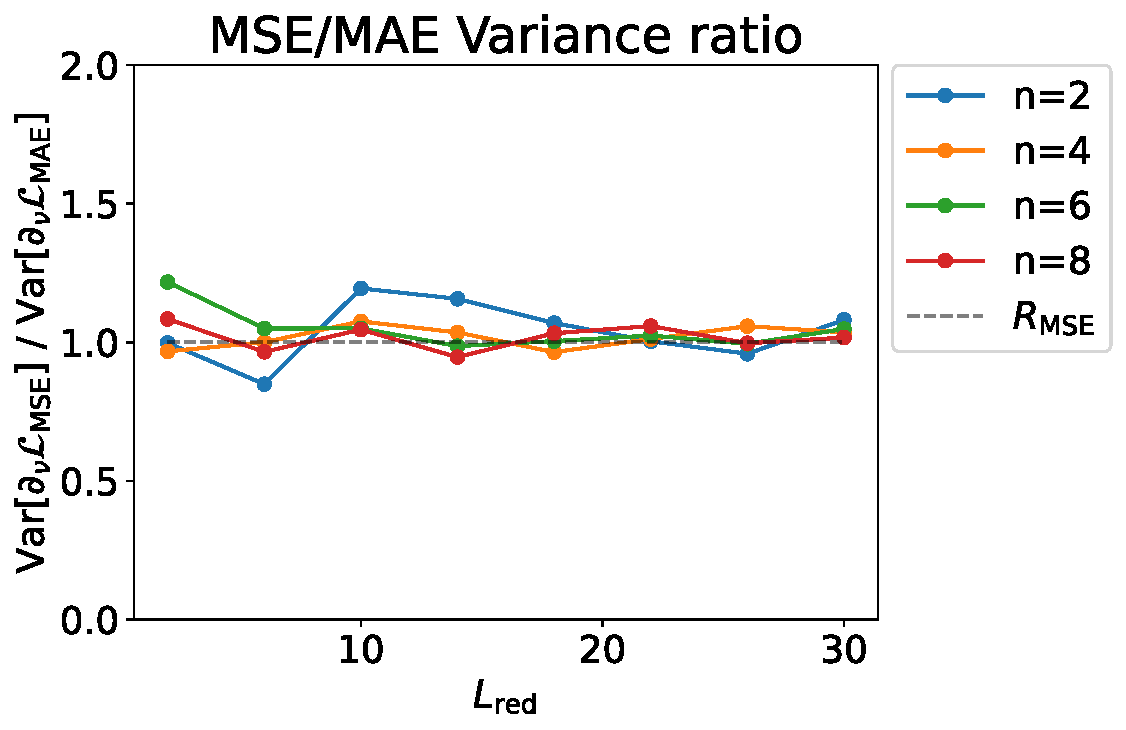
\includegraphics[width=7cm]{variance-mse-mae-ratio_encoding3.pdf}
                \caption{破線は近似比 $R_{\mathrm{MSE}}=1$ を表す}
            \end{figure}
        \end{column}
        \begin{column}{0.5\textwidth}
            \begin{small}
                \centering\hspace*{-10pt} $\Var_{V(\bth)}[\pd_{\theta_\nu}\calL_{\mathrm{LOG}}(\bth)]\,/\,\Var_{V(\bth)}[\pd_{\theta_\nu}\calL_{\mathrm{MAE}}(\bth)]$
            \end{small}
            \begin{figure}
                \centering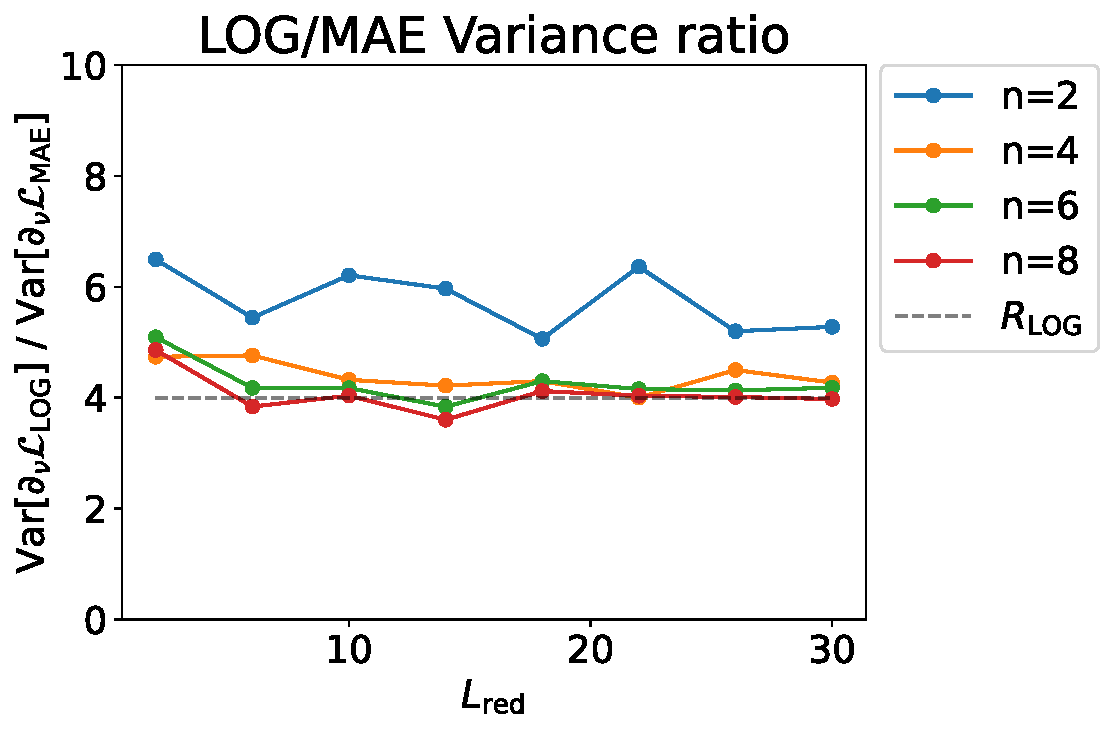
\includegraphics[width=7cm]{variance-log-mae-ratio_encoding3.pdf}
                \caption{破線は近似比 $R_{\mathrm{LOG}}=4$ を表す}
            \end{figure}
        \end{column}
    \end{columns}
    \centering
    % \hspace{-10pt}数値計算では、学習回路が浅くても近似比に近い値をとっている。
    \hspace{-10pt}数値計算では、学習回路が浅くても誤差関数によらず勾配の分散のスケーリングはほぼ同じ\\
    
    \begin{scriptsize}
        (アヤメのデータセットを用いてコスト関数を定義した。)
    \end{scriptsize}
\end{frame}




\section{まとめ}
\begin{frame}{まとめ}
    \vspace*{-20pt}
    \hspace*{-50pt}

    \begin{center}
        {\large\colorbox{blue!40}{\makebox[23em]{バレンプラトーに対するデータ入力の影響の研究}}}
    \end{center}

    \begin{itemize}
        \item コスト関数の勾配の分散の上界をデータ入力の観点から導出し、数値的にも検証
        \item データ入力後の状態のエンタングルメントや入力回路の表現能力が大きい\\ → 上界が小さくなり、バレンプラトーにつながる
        \item データ入力の層数が$O(\log{n})$なら、上界のスケーリングは指数関数的ではない
        \item 入力データがガウス分布に従う場合、データの分散が勾配の分散の下界において重要
        \item 勾配の分散のスケーリングは、誤差関数の形にほぼ依存しないことを数値的に確認
    \end{itemize}

    \begin{center}
        {\large\colorbox{blue!40}{\makebox[15em]{今後の課題}}}
    \end{center}

    \begin{itemize}
        \item より一般的な入力回路において、コスト関数の勾配の分散の下界を調べる。
        \item 汎化性能の観点からも入力回路について考慮する。(今回は訓練可能性のみ)
        \item 古典計算が計算量的に難しい入力回路になっているか
    \end{itemize}
    % スケーリングが分かれば、ある設定に対してかかりうる計算量の下限を推定できる。
\end{frame}



\appendix



\begin{frame}{オブザーバブルの局所性について}
    ローカルオブザーバブル
    \begin{itemize}
        \item $Z_1 := Z \ot \bbid \ot \bbid \ot \cdots \ot \bbid$
        \item $\dyad{0}_1 = (Z_1 + \bbid_1)/2$
        \item $O_L := \frac1n \sum_{j=1}^{n}\dyad{0}_{j} \otimes \bbid_{\bar{j}}$(ローカルオブザーバブルの線形和)
        \item 学習回路の深さが $\order{\log{n}}$ 程度ならバレンプラトーは起きない。
    \end{itemize}
    
    グローバルオブザーバブル
    \begin{itemize}
        \item $Z\otn{n} := Z \ot Z \ot \cdots \ot Z$
        \item 学習回路の深さによらずバレンプラトーを引き起こす。
    \end{itemize}
\end{frame}



\begin{frame}{ユニタリ $t$--デザイン}
    % ユニタリの集合$\{U_k\}_k$による多項式$P_{2,2}(U)$の平均が、ハール分布による平均と等しいとき、$\{U_k\}_k$はユニタリ$2$デザインであるという. (ex. $P_{2,2}(U) = U\dg AUBU\dg CU$)
    \begin{definition}
        $P_{t,t}(U)$ は、ユニタリ $U$ と $U\dg$ のそれぞれの成分に関して最大次数 $t$ の斉次多項式とする。$K$ 個のユニタリの集合 $\{U_k\}$ が以下の条件を満たすとき、この集合はユニタリ $t$--デザインを成すという。(例:$P_{t,t}(U) = U\dg AUBU\dg CU$)
        \begin{align*}
            \frac1K \sum_{k=1}^{K} P_{t}(U_k) = \int_{\calU(d)}P_{t} (U) d\mu(U)
        \end{align*}
    \end{definition}

    \begin{itemize}
        \item パウリ群:$\mathcal{P}(n)=\{e^{i\frac{k\pi}{2}}\, P_{j_1}\otimes \cdots\otimes P_{j_n}| k,j_l=0,1,2,3\}$ はユニタリ $1$ デザイン
        \item クリフォード群:$\mathcal{C}(n)=\{U\in \mathcal{U}(2^n)|\,UPU^\dagger = \mathcal{P}(n)\}$ はユニタリ $3$ デザイン
        \item もし $\{U_k\}$ がユニタリ $t$--デザインならば、ユニタリ $(t-1)$--デザインでもある。
    \end{itemize}

    % \begin{figure}
    %     \begin{center}
    %         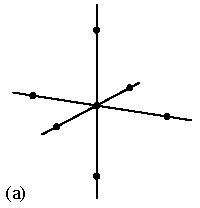
\includegraphics[height=3.5cm,width=4cm]{1-design.pdf}
    %         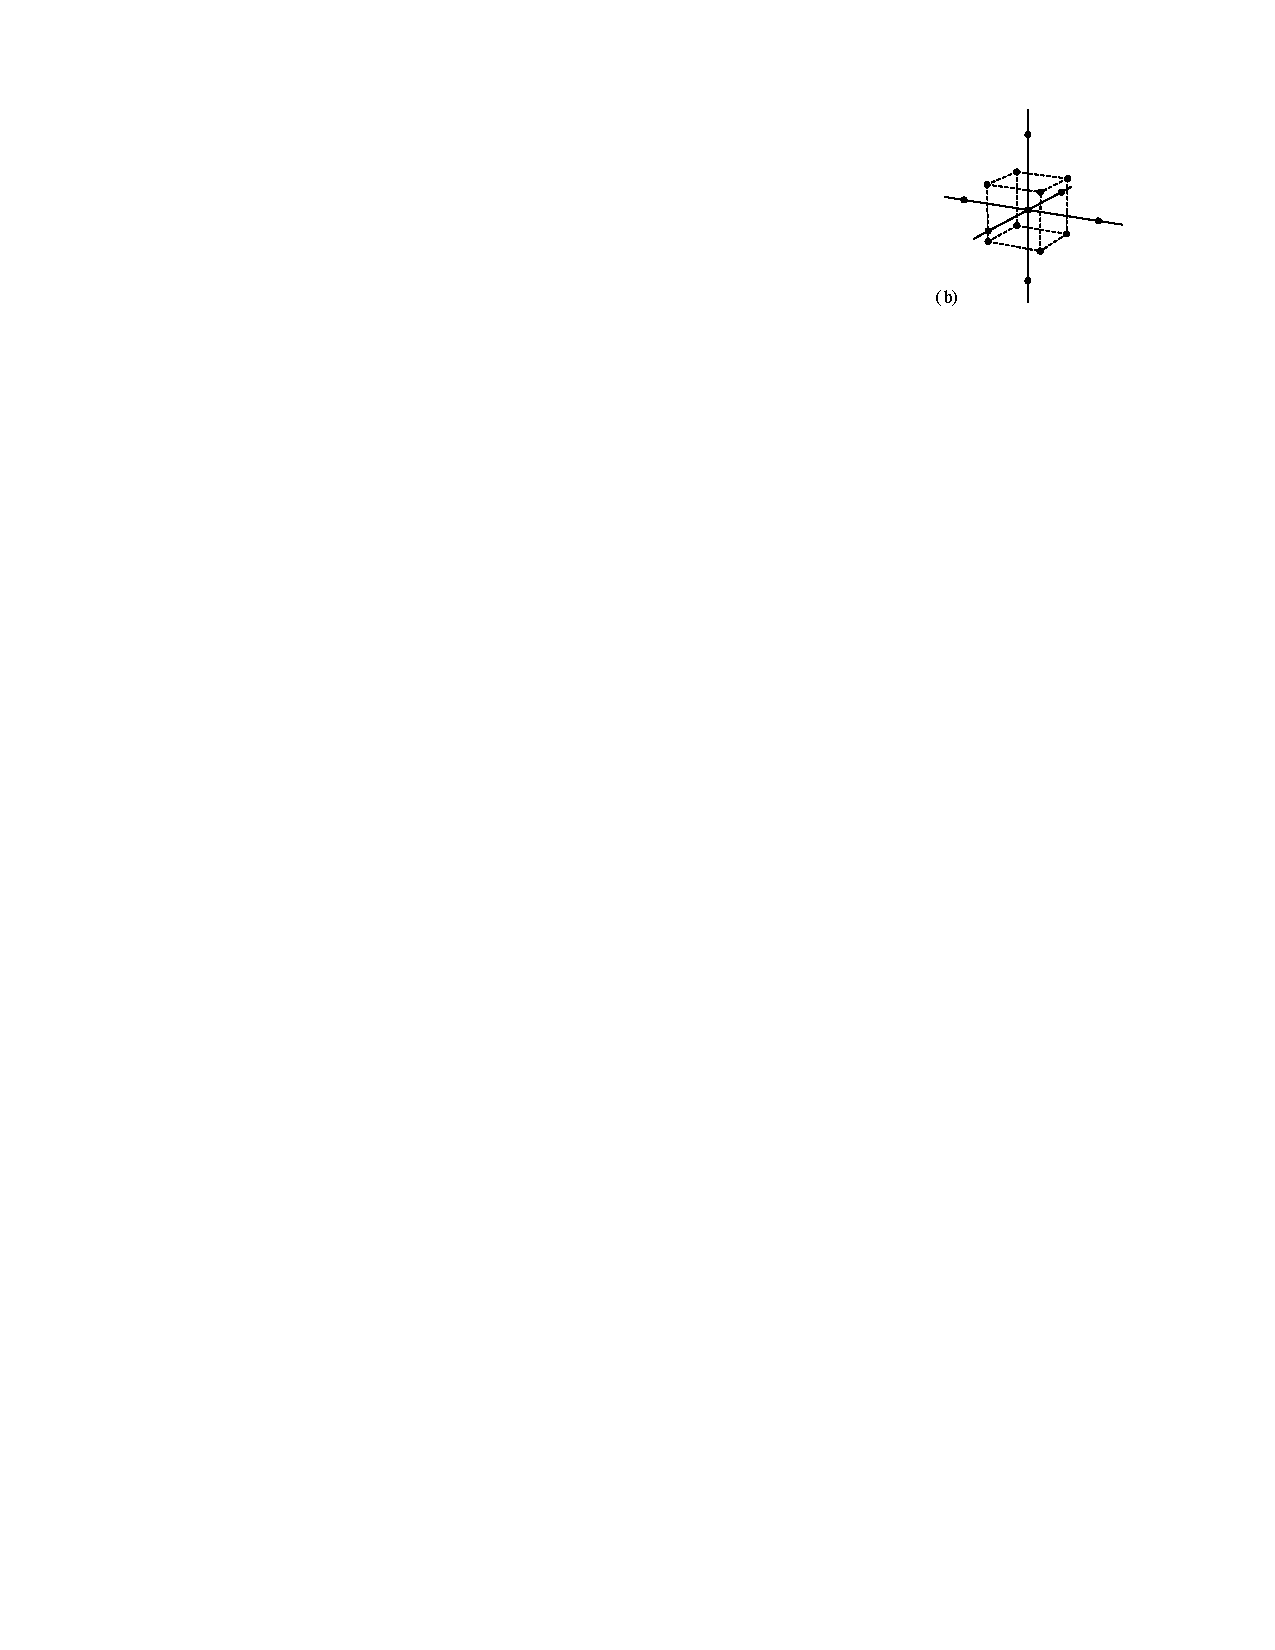
\includegraphics[height=3.5cm,width=4cm]{2-design.pdf}
    %         \caption{左: ユニタリ$1$デザイン, 右: ユニタリ$2$デザイン\cite{gross2007evenly}}
    %     \end{center}
    % \end{figure}
\end{frame}




\begin{frame}{バレンプラトーの回避方法}
    \begin{itemize}
        \item (データ入力なしの場合)ローカルオブザーバブルを用いることより、学習回路の深さが $\order{\log{n}}$ であればバレンプラトーは起きないことが示されている。%\cite{cerezo2021cost}
        \item 学習回路の各層ごとにパラメーターを最適化する。これにより、実質的な学習回路の深さを減らすことができる。%\cite{skolik2021layerwise}
        \item 一部の学習パラメーターの初期値を残りの回路と打ち消し合うように設定する。これにより、実質的な学習回路の深さを減らすことができる。%\cite{grant2019initialization}
        \item 学習パラメーター間に相関を持たせる。これにより、学習回路の表現能力を抑えることができる。%\cite{holmes2022connecting}
        \item 学習パラメーターの初期値を、一様分布ではなく、正規分布からサンプリングする。%\cite{zhang2022escaping}
    \end{itemize}
\end{frame}




\definecolor{circleColor}{RGB}{100,180,44}   % Green
\definecolor{ellipseColor}{RGB}{65,160,241}  % Blue
\begin{frame}{量子回路の表現力:定義}
    量子回路の表現力とは次のように定義される。
    \begin{align*}
        \epsilon_{\bbU}^{(t,p)}(X) &:= \norm{A^{(t)}_{\bbU}(X)}_p,\\
        \calA_{\bbU}^{(t)}(X) &:= \int_{{\color{circleColor} \calU(d)}} d\mu_{\Haar}(V)\,V\otn{t}X\otn{t}(V\otn{t})\dg - \int_{{\color{ellipseColor} \bbU}} dU\,U\otn{t}X\otn{t}(U\otn{t})\dg.
    \end{align*}

    \begin{columns}
        \hspace*{40pt}
        \begin{column}{0.5\textwidth}
            \begin{itemize}
                \item $\norm{\cdot}_p$:シャッテン $p$--ノルム
                \item $X$:初期状態$\dyad{0}^{\otimes n}$
                \item $\calU(d)$:次元$d$のユニタリ群
                \item $t=2$の場合を考える
            \end{itemize}
        \end{column}

        \begin{column}{0.5\textwidth}
            \begin{figure}[H]
                \centering
                \begin{tikzpicture}[scale=0.5]
                    \definecolor{circleColor}{RGB}{100,180,44}   % Green
                    \definecolor{ellipseColor}{RGB}{65,160,241}  % Blue
                    % Draw the circle
                    \draw[fill=circleColor, draw=black] (0,0) circle (3.2cm);
                    % Add text inside the circle
                    \node at (0,1.5) {\small Unitary group $\calU(d)$};
                  
                    % Draw the ellipse inside the circle
                    \draw[fill=ellipseColor, draw=black] (-0.5,-0.9) ellipse (2.5cm and 1.5cm);
                    % Add text inside the ellipse
                    \node at (-0.5,-0.9) {\small Accesible set $\bbU$};
                  \end{tikzpicture}
                \caption{量子回路の表現領域}
            \end{figure}
        \end{column}
    \end{columns}
\end{frame}


\begin{frame}{量子回路の表現力:回路の例}
    \begin{columns}
        \begin{column}{0.5\textwidth}
            \centering\hspace*{-30pt} Tensor Product Ansatz の表現力
            \begin{tikzpicture}
                \node[scale=0.55]{
                \begin{quantikz}
                    \lstick{$\ket{0}$}\slice{} & \gate{R_x} & \gate{R_y}\slice{1}& \gate{R_x} & \gate{R_y}\slice{2}& \gate{R_x} & \gate{R_y}\slice{3}& \meter{}\\
                    \lstick{$\ket{0}$}      & \gate{R_x} & \gate{R_y}      & \gate{R_x} & \gate{R_y}      & \gate{R_x} & \gate{R_y}      & \meter{}\\
                    \lstick{$\ket{0}$}      & \gate{R_x} & \gate{R_y}      & \gate{R_x} & \gate{R_y}      & \gate{R_x} & \gate{R_y}      & \meter{}\\
                    \lstick{$\ket{0}$}      & \gate{R_x} & \gate{R_y}      & \gate{R_x} & \gate{R_y}      & \gate{R_x} & \gate{R_y}      & \meter{}\\
                    \lstick{$\ket{0}$}      & \gate{R_x} & \gate{R_y}      & \gate{R_x} & \gate{R_y}      & \gate{R_x} & \gate{R_y}      & \meter{}\\
                    \lstick{$\ket{0}$}      & \gate{R_x} & \gate{R_y}      & \gate{R_x} & \gate{R_y}      & \gate{R_x} & \gate{R_y}      & \meter{}
                \end{quantikz}
                };
            \end{tikzpicture}
        \end{column}
        
        \begin{column}{0.5\textwidth}
            \centering\hspace*{-30pt} Alternating Layered Ansatz の表現力
            \begin{tikzpicture}
                \node[scale=0.55]{
                \begin{quantikz}
                    \lstick{$\ket{0}$}\slice{}&\gate{R_x}&\gate{R_y}&\ctrl{1}\slice{1}&\qw       &\qw       &\qw\slice{2}&\gate{R_x}&\gate{R_y}&\ctrl{1}\slice{3}& \meter{}\\
                    \lstick{$\ket{0}$}        &\gate{R_x}&\gate{R_y}&\targ{}          &\gate{R_x}&\gate{R_y}&\ctrl{1}    &\gate{R_x}&\gate{R_y}&\targ{}          & \meter{}\\
                    \lstick{$\ket{0}$}        &\gate{R_x}&\gate{R_y}&\ctrl{1}         &\gate{R_x}&\gate{R_y}&\targ{}     &\gate{R_x}&\gate{R_y}&\ctrl{1}         & \meter{}\\
                    \lstick{$\ket{0}$}        &\gate{R_x}&\gate{R_y}&\targ{}          &\gate{R_x}&\gate{R_y}&\ctrl{1}    &\gate{R_x}&\gate{R_y}&\targ{}          & \meter{}\\
                    \lstick{$\ket{0}$}        &\gate{R_x}&\gate{R_y}&\ctrl{1}         &\gate{R_x}&\gate{R_y}&\targ{}     &\gate{R_x}&\gate{R_y}&\ctrl{1}         & \meter{}\\
                    \lstick{$\ket{0}$}        &\gate{R_x}&\gate{R_y}&\targ{}          &\qw       &\qw       &\qw         &\gate{R_x}&\gate{R_y}&\targ{}          & \meter{}
                \end{quantikz}
                };
            \end{tikzpicture}
        \end{column}
    \end{columns}
\end{frame}


\begin{frame}{量子回路の表現力:プロット}
    \begin{columns}
        \begin{column}{0.5\textwidth}
            \centering\hspace*{-30pt} Tensor Product Ansatz の表現力
            \begin{figure}
                \centering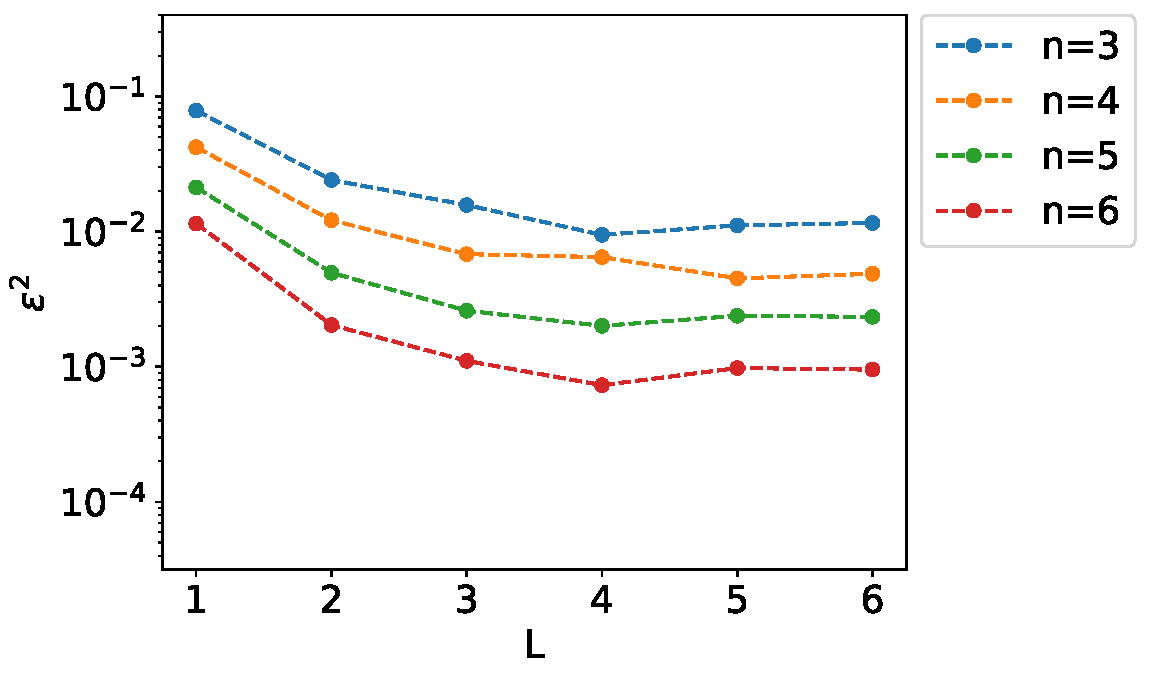
\includegraphics[width=7cm]{product-circuit-exp.pdf}
            \end{figure}
        \end{column}
        
        \begin{column}{0.5\textwidth}
            \centering\hspace*{-30pt} Alternating Layered Ansatz の表現力
            \begin{figure}
                \centering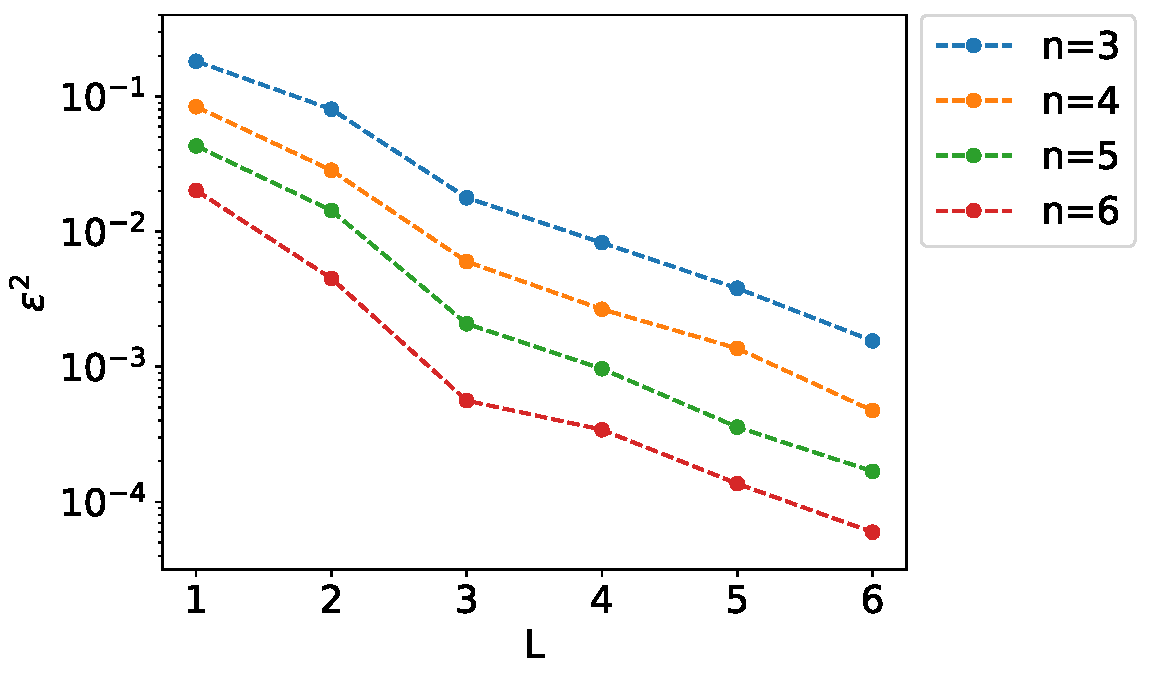
\includegraphics[width=7cm]{alt-circuit-exp.pdf}
            \end{figure}
        \end{column}
    \end{columns}
\end{frame}




\begin{frame}{上界の具体的な形}
    $$
        y_i \in \{0,1\},\quad \colorbox{orange!30}{$\ell_i(\bth)$} := \Tr[\rho_i(\bth)\,O_\rmL] \in [0,1],\quad
        \colorbox{green!30}{$\calL(\bth)$} := \frac1N\sum_{i=1}^N f(y_i, \colorbox{orange!30}{$\ell_i(\bth)$})
    $$
    \begin{theorem}
        量子機械学習におけるコスト関数の勾配の分散の上界
        \begin{align*}
            &\Var_{\bth}[\pd_{\theta_\nu} \colorbox{green!30}{$\calL(\bth)$}]\\
            &\leq A_f \times r_{n,s} \times \bar{D}_{\mathrm{HS}}\\
            &=
            2\max_{i,\bth} [(\pd_{\ell_i(\bth)}f)^2]
            \times \frac{2^{2s-1}}{(2^{2s}-1)^2}\qty(\Tr[(O_\rmL^h)^2] - \frac{\Tr[O_\rmL^h]^2}{2^s})
            \times \int_{\bbU}dU D_{\mathrm{HS}} ( \rho^{(h)},\, \bbI/2^s )
        \end{align*}
        ただし、$O_\rmL^h = \Tr_{\bar{h}}[O_\rmL]$
    \end{theorem}
\end{frame}




\begin{frame}{スライド~\ref{qml-var-alt}の学習回路}
    \begin{columns}
        \begin{column}{0.5\textwidth}
        1量子ビットのユニタリ $2$--デザイン
        \begin{figure}[H]
            \centering
            \begin{tikzpicture}
                \node[scale=1]{
                    \begin{quantikz}
                        \qw & \gate[wires=1,style={fill=red!50}][1cm][0.7cm]{}& \qw
                    \end{quantikz}
                    \begin{quantikz}
                        {\LARGE \textbf{=}}
                    \end{quantikz}
                    \begin{quantikz}
                        \qw\slice{} & \gate{R_x} &\gate{R_y}\slice{$\times 10$} & \qw
                    \end{quantikz}
                    };
            \end{tikzpicture}
            \caption{TPA のゲートブロックとして用いた構造}
            \label{fig:tpa-example}
        \end{figure}
        \end{column}
        
        \begin{column}{0.5\textwidth}
            \begin{figure}[H]
                \centering
                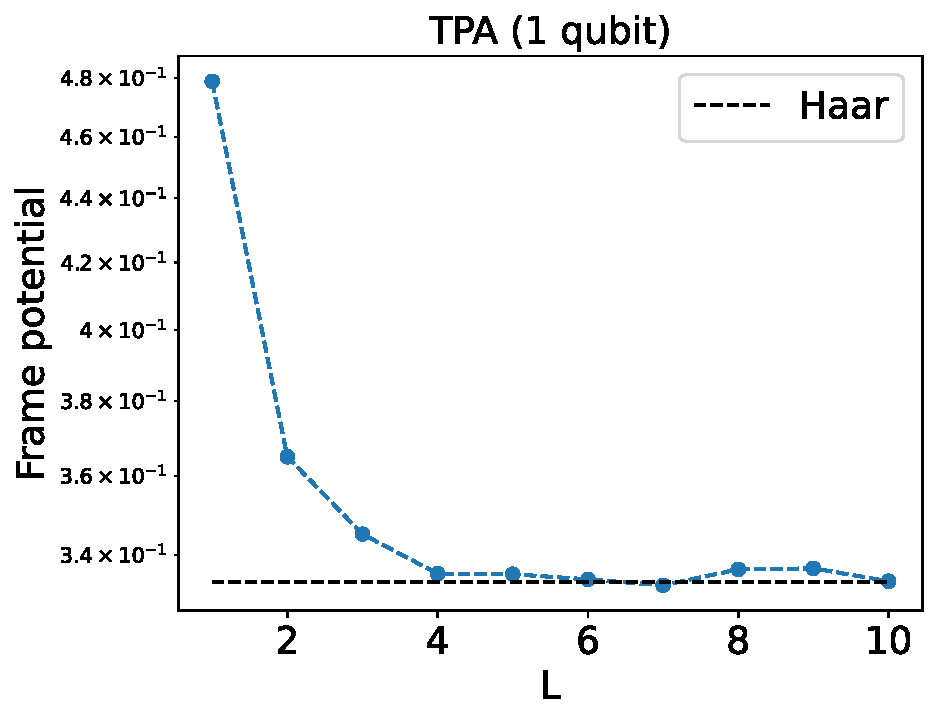
\includegraphics[width=6cm]{1qubit-tpa-exp.pdf}
                \caption{1量子ビットの Tensor Product Ansatz のフレームポテンシャル。黒の破線は1量子ビットがユニタリ $2$--デザインを成す場合のフレームポテンシャル($=1/3$)である。}
                \label{fig:1qubit-tpa-exp}
            \end{figure}
        \end{column}
    \end{columns}
\end{frame}




\begin{frame}{コスト関数の勾配の分散の下界:考察}
    極端な例として、ラベル $0$ に属する入力データ $\calX = \{\bs{x}\}$ と ラベル $1$ に属する入力データ $\calZ = \{\bs{z}\}$ が $\calX = \calZ$ である場合を考える。
    このとき
    \begin{alignat*}{2}
        \calL_{\mathrm{MAE}}(\bth)
        &= \frac1N\Big(\sum_{x\in\calX} |\ell_{i}(\bth) - 0| &&+ \sum_{z\in\calZ} |\ell_{i}(\bth) - 1|\Big)\\
        &= \frac1N\Big(\sum_{x\in\calX} \ell_{i}(\bth)       &&+ \sum_{x\in\calX} (1 - \ell_{i}(\bth))\Big) = \frac12
    \end{alignat*}
    
    ゆえに、コスト関数の勾配は $0$ となり、分散も $0$ となる。\\

    → 入力回路の構造が極めて単純であっても、異なるラベル間の入力データが近いほど、\\
    コスト関数の勾配の分散は小さくなると考えられる。
\end{frame}

\begin{frame}{コスト関数の勾配の分散の下界:$\calL_{\mathrm{MSE}}(\bth)$ の考察}
    極端な例として、ラベル $0$ に属する入力データ $\calX = \{\bs{x}\}$ と ラベル $1$ に属する入力データ $\calZ = \{\bs{z}\}$ が $\calX = \calZ$ である場合を考える。
    このとき
    \begin{alignat*}{2}
        \calL_{\mathrm{MSE}}(\bth)
        &= \frac1N\Big(\sum_{x\in\calX} (\ell_{i} - 0)^2 &+ \sum_{x\in\calX} (\ell_{i} - 1)^2\Big)\\
        &= \frac1N\Big(\sum_{x\in\calX} \ell_{i}^2       &+ \sum_{x\in\calX} (\ell_{i} - 1)^2\Big)\\
        &= \frac12 + \frac1N\sum_{x\in\calX} 2\qty(\ell_i - \frac12)^2
    \end{alignat*}
    
    このとき、$\ell_i$ が $\frac12$ のときにコスト関数 $\calL_{\mathrm{MSE}}(\bth)$ は最小となるため、教師ラベル $y_i = \{0,1\}$ に近づくことはない。
\end{frame}

\begin{frame}{コスト関数の勾配の分散の下界:$\calL_{\mathrm{LOG}}(\bth)$ の考察}
    極端な例として、ラベル $0$ に属する入力データ $\calX = \{\bs{x}\}$ と ラベル $1$ に属する入力データ $\calZ = \{\bs{z}\}$ が $\calX = \calZ$ である場合を考える。
    このとき
    \begin{align*}
        \calL_{\mathrm{LOG}}(\bth)
        &= \frac1N\Big(\sum_{x\in\calX} -\log(1-\ell_i) + \sum_{x\in\calX} -\log(\ell_i)\Big)\\
        &= \frac1N\Big(\sum_{x\in\calX} - \log\ell_i(1-\ell_i)\Big)\\
        &= \frac1N\Big(\sum_{x\in\calX} - \log\qty[-\qty(\ell_i - \frac12)^2 + \frac14]\Big)
    \end{align*}
    
    このとき、$\ell_i$ が $\frac12$ のときにコスト関数 $\calL_{\mathrm{LOG}}(\bth)$ は最小となるため、教師ラベル $y_i = \{0,1\}$ に近づくことはない。
\end{frame}


\end{document}

